%% Finistral AI: Financial Sentiment Analyst
%% Formatted for GR Journals Submission Template
%% Compile with: pdflatex finistral_grjournals.tex (run twice for cross-references)

\documentclass[a4paper]{article}

%%% ==== Page Layout ====
\usepackage[top=1in, bottom=1in, left=1in, right=1in]{geometry}

%%% ==== Fonts (pdfLaTeX) ====
\usepackage[T1]{fontenc}
\usepackage{newtxtext,newtxmath}   % Times New Roman clone
\usepackage{carlito}               % Carlito = metric-compatible Calibri substitute
\newcommand{\calibrifont}{\fontfamily{Crlt-LF}\selectfont}

%%% ==== Packages ====
\usepackage{setspace}
\usepackage{titlesec}
\usepackage{booktabs}
\usepackage{graphicx}
\usepackage{hyperref}
\usepackage{url}
\usepackage{amsmath}  % amssymb already provided by newtxmath
\usepackage{caption}
\usepackage{enumitem}
\usepackage{xcolor}
\usepackage{subcaption}

%%% ==== Revision placeholder for numbers awaiting decontaminated re-run ====

%%% ==== Body text: TNR 10.5pt, single spacing, justified ====
\renewcommand{\normalsize}{\fontsize{10.5}{12.6}\selectfont}
\normalsize
\singlespacing

%%% ==== Section Formatting (TNR 10.5pt Bold, numbered) ====
\titleformat{\section}
  {\fontsize{10.5}{12.6}\selectfont\bfseries}
  {\thesection.}{0.5em}{}
\titlespacing*{\section}{0pt}{12pt}{6pt}

\titleformat{\subsection}
  {\fontsize{10.5}{12.6}\selectfont\bfseries}
  {\thesubsection}{0.5em}{}
\titlespacing*{\subsection}{0pt}{10pt}{4pt}

\titleformat{\subsubsection}
  {\fontsize{10.5}{12.6}\selectfont\bfseries}
  {\thesubsubsection}{0.5em}{}
\titlespacing*{\subsubsection}{0pt}{8pt}{4pt}

%%% ==== Custom Commands for GR Journals ====
% Title: Calibri 20pt, Bold, left-aligned
\newcommand{\grtitle}[1]{%
  {\calibrifont\fontsize{20}{24}\selectfont\bfseries\raggedright #1\par}%
  \vspace{6pt}%
}

% Author line: TNR 10pt
\newcommand{\grauthor}[1]{%
  {\fontsize{10}{12}\selectfont #1\par}%
}

% Affiliation: TNR 9pt, Italic
\newcommand{\graffiliation}[1]{%
  {\fontsize{9}{11}\selectfont\itshape #1\par}%
}

% Email: TNR 9pt
\newcommand{\gremail}[1]{%
  {\fontsize{9}{11}\selectfont #1\par}%
}

% Abstract heading: Calibri 12pt, Bold
\newcommand{\grabstractheading}{%
  \vspace{12pt}%
  {\calibrifont\fontsize{12}{14.4}\selectfont\bfseries Abstract\par}%
  \vspace{4pt}%
}

% Abstract text: Calibri 10.5pt, single spacing
\newenvironment{grabstract}{%
  \calibrifont\fontsize{10.5}{12.6}\selectfont\singlespacing
}{\par\vspace{6pt}}

% Keywords: TNR 9pt, Italic
\newcommand{\grkeywords}[1]{%
  {\fontsize{9}{11}\selectfont\textit{Keywords}: \textit{#1}\par}%
  \vspace{12pt}%
}

%%% ==== Hyperref Setup ====
\hypersetup{
  colorlinks=true,
  linkcolor=blue,
  citecolor=blue,
  urlcolor=blue,
  bookmarks=true,
  pdfauthor={Zainab Mirza, Ayan J. Shaikh, Fazal Jalil Parkar},
  pdftitle={Finistral AI: An Efficient Financial-Sentiment LoRA Adapter and a Train/Test Contamination Case Study}
}

%%% ==== Caption Setup ====
\captionsetup{font=small, labelfont=bf}
\captionsetup[figure]{name={Fig.}}

\pagestyle{plain}

%%% ================================================================
\begin{document}

%%% ==== Title Block ====
\grtitle{Finistral AI: An Efficient Financial-Sentiment LoRA Adapter and a Train/Test Contamination Case Study}

\grauthor{Zainab Mirza\textsuperscript{1}, Ayan Javeed Shaikh\textsuperscript{2,*}, Fazal Jalil Parkar\textsuperscript{3}}

\vspace{4pt}
\graffiliation{\textsuperscript{1}University of Mumbai, Mumbai, Maharashtra, India}
\graffiliation{\textsuperscript{2}Indiana University Bloomington, Bloomington, IN 47405, USA}
\graffiliation{\textsuperscript{3}Tata Consultancy Services (TCS), India}

\vspace{2pt}
\gremail{\textsuperscript{*}Email: ayshaikh@iu.edu}

%%% ==== Abstract ====
\grabstractheading
\begin{grabstract}
We present Finistral-7B-LoRA, a parameter-efficient financial-sentiment classifier produced by applying Low-Rank Adaptation (LoRA) to the 7-billion-parameter Mistral-7B-v0.1 language model. The adapter is trained on the open-source FinGPT/fingpt-sentiment-train corpus of approximately 77,000 labelled sentences, updating $\approx$\,0.58\,\% of the model parameters ($\approx$\,41.9\,M trainable, matching the released adapter's configuration), on two NVIDIA A100 (40\,GB) GPUs of Indiana University's Big Red 200 supercomputer. On the full Financial PhraseBank \texttt{sentences\_allagree} split the adapter shows an apparent 99.56\,\% accuracy, but our own data-overlap audit reveals that 75.2\,\% of those evaluation sentences appear \emph{verbatim}, with identical gold labels, inside the training corpus, so that figure reflects memorisation rather than generalisation and is retained only as a contamination diagnostic. The paper's primary evidence is instead a corrected, exact-match-decontaminated evaluation: on the 560-sentence decontaminated Financial PhraseBank remainder Finistral attains 98.9\,\% accuracy, on FiQA-SA 87.7\,\% accuracy / 0.883 weighted F1, and on Twitter Financial News Sentiment 78.9\,\% accuracy / 0.796 weighted F1. These figures are statistically indistinguishable from the strongest FinGPT-class adapter on each dataset and significantly ahead of FinBERT off-distribution, with all comparisons carrying per-example significance tests. Our main contributions are (i) an efficient, fully reproducible single-node LoRA recipe for financial sentiment whose adapter runs inference on a single GPU, and (ii) a cautionary evaluation/contamination case study quantifying how corpus overlap and evaluation-harness defects can simultaneously inflate a model and deflate its baselines in the financial-NLP literature. The released adapter (Ayansk11/Finistral-7B\_lora on Hugging Face), decontamination and evaluation scripts, and frozen evaluation sets make every reported evaluation number independently reproducible.
\end{grabstract}

\grkeywords{financial sentiment analysis, Low-Rank Adaptation (LoRA), parameter-efficient fine-tuning (PEFT), Mistral-7B, large language models, FinGPT, Financial PhraseBank}

%%% ==== Graphical Abstract ====
\begin{figure}[h!]
\centering
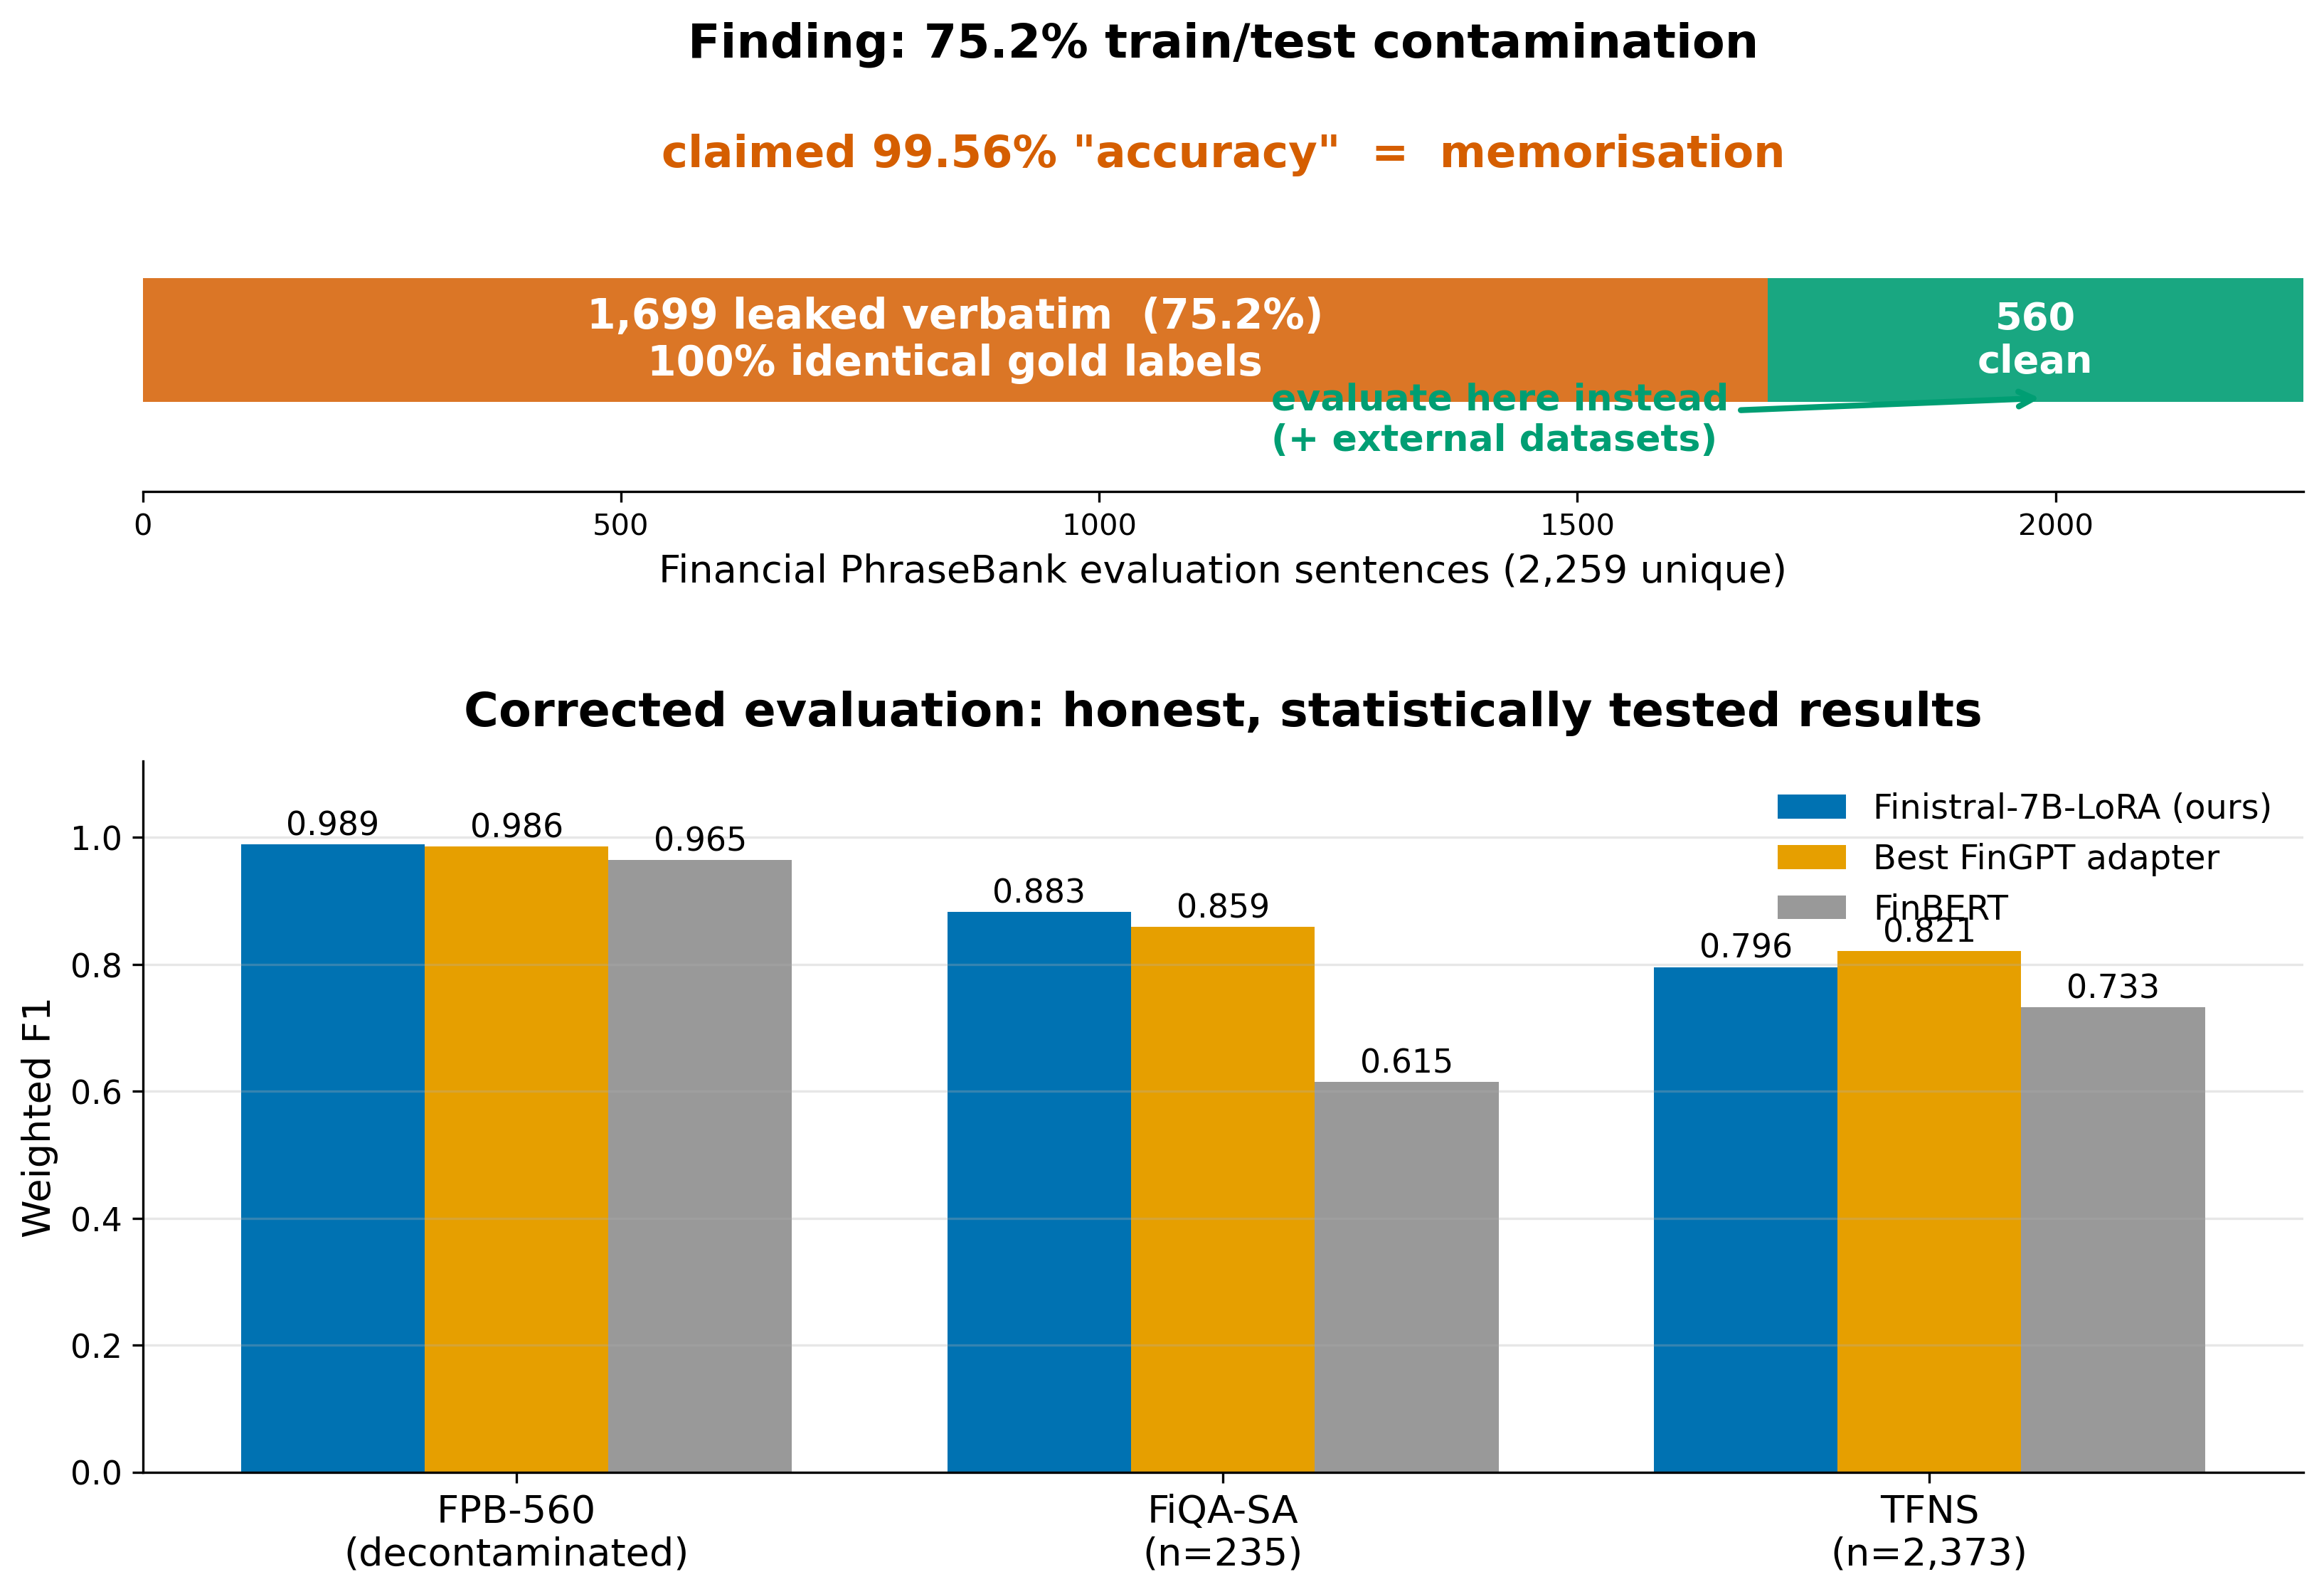
\includegraphics[width=\textwidth]{figures/graphical_abstract.png}
\caption*{Top: 75.2\,\% of the Financial PhraseBank evaluation set appears verbatim, with identical gold labels, in the fine-tuning corpus, so the originally claimed 99.56\,\% accuracy reflects memorisation. Bottom: the corrected evaluation on the exact-match-decontaminated remainder and two external datasets, with per-example significance tests (Section~\ref{sec:contamination}).}
\end{figure}

%%% ==== Novelty Statement ====
\noindent{\fontsize{9}{11}\selectfont\itshape Novelty Statement:
This work contributes (i) an efficient, fully reproducible LoRA recipe for adapting the compute-efficient Mistral-7B backbone to financial sentiment classification, updating only $\approx$\,0.58\,\% of the model parameters, and (ii) a contamination-and-evaluation case study: we show that the widely used FinGPT sentiment corpus overlaps the Financial PhraseBank benchmark by 75.2\,\% at the sentence level (identical labels), and that common evaluation-harness defects can drive instruction-tuned baselines below their majority-class floor. We release the adapter, decontamination scripts, and a corrected evaluation harness to enable low-cost, leakage-aware FinNLP research.\par}

\vspace{12pt}

%%% ================================================================
%%% MAIN BODY
%%% ================================================================

\section{Introduction}

Financial markets digest a relentless stream of earnings releases, macro-economic announcements, social-media chatter, and regulatory filings. Traders and risk managers depend on sentiment analysis systems that can transform this unstructured text into structured signals, typically the triplet positive, neutral, or negative within seconds. Conventional rule-based lexicons \cite{loughran2011} and classical machine-learning pipelines capture obvious polarity cues, yet they struggle with the domain's specialised jargon (``EPS miss''), pragmatic hedges (``guidance was raised but remains below expectations''), and rapidly evolving slang from forums such as WallStreetBets.

Large language models (LLMs) have recently set new performance bars on general-domain sentiment tasks, but two obstacles limit their usefulness in finance:

\textbf{Domain mismatch:} Out-of-the-box LLMs misinterpret sector-specific expressions and implicit market context.

\textbf{Compute cost:} Full fine-tuning of multi-billion-parameter models demands prohibitive GPU hours and storage, placing them out of reach for most academic or boutique-fund settings.

Parameter-Efficient Fine-Tuning (PEFT) techniques such as Low-Rank Adaptation (LoRA) \cite{hu2022} address both issues by inserting small trainable matrices into each transformer layer while freezing the backbone. This yields two attractive properties: (i) the modified model can be trained on a single commodity GPU, and (ii) the resulting adapter file is lightweight, making deployment trivial.

\subsection{Research Questions}

We investigate whether a LoRA-based adaptation of the compute-efficient Mistral-7B decoder can provide competitive financial sentiment classification under a contamination-audited, exact-match-decontaminated evaluation protocol:

\textbf{Research Question 1:} Once train/test contamination is removed and a corrected evaluation harness is used, how does a LoRA-tuned Mistral-7B compare with specialised encoders such as FinBERT and existing FinGPT adapters on Financial PhraseBank and on external financial-sentiment datasets?

\textbf{Research Question 2:} Does the PEFT recipe retain training- and inference-time efficiency suitable for realistic academic or start-up budgets?

\textbf{Research Question 3:} How much of the apparent performance of FinGPT-corpus-trained sentiment models on Financial PhraseBank is attributable to train/test overlap rather than to genuine generalisation?

\subsection{Our Approach}

To answer these questions, we built Finistral-7B-LoRA. The adapter is trained on the publicly available FinGPT/fingpt-sentiment-train corpus (${\sim}$77\,k labelled sentences) and validated on a 5\,\% hold-out split. Training runs for four epochs on two A100 (40\,GB) GPUs of Indiana University's Big Red 200 supercomputer, updating $\approx$\,0.58\,\% of the model parameters ($\approx$\,41.94\,M). Validation loss bottomed out at 0.1009 after epoch 2 and began to rise thereafter, so that checkpoint is used for all downstream evaluations. Because Financial PhraseBank is itself one of the constituent sources of the FinGPT corpus, we additionally audit the train/test overlap and re-evaluate on a decontaminated subset and on external datasets (Section~\ref{sec:contamination}).

\subsection{Contributions}

Our work makes the following contributions:

\textbf{Reproducible efficient recipe \& model release:} We publish Finistral-7B-LoRA (an 83.9\,MB fp16 adapter over Mistral-7B-v0.1, 41{,}943{,}040 trainable parameters $\approx$\,0.58\,\% of the backbone; the file size itself verifies the count, $41.94\,\mathrm{M} \times 2$\,bytes $= 83.9$\,MB), tokeniser files, and the complete training, decontamination, and evaluation scripts, so that every number in this paper can be reproduced end-to-end on a single node.

\textbf{Contamination \& evaluation case study:} We quantify a 75.2\,\% verbatim, identically-labelled overlap between the FinGPT training corpus and the Financial PhraseBank \texttt{sentences\_allagree} evaluation set, and show how a set of common harness defects (right-padding on decoder-only models, a \texttt{max\_length}/\texttt{padding} collision, a single mismatched prompt template, and a neutral-defaulting parser) can drive instruction-tuned baselines below their majority-class floor. We report corrected results on an exact-match-decontaminated subset and on external datasets.

\textbf{Efficiency analysis:} We demonstrate that financial sentiment adapters can be trained in $<$\,1 GPU-hour per epoch and deployed with minimal memory overhead, opening the door to low-cost, reproducible FinNLP research.


\section{Related Work}

Early attempts at financial sentiment analysis relied on domain-specific lexicons such as the Loughran--McDonald word lists \cite{loughran2011}, which classify words by their usage in financial filings into negative, positive, and further tone categories such as uncertainty and litigiousness. Although lexicon rules are transparent, their coverage is limited and they struggle with figurative or contextual language. Subsequent classical machine-learning pipelines trained support-vector or recurrent networks on Financial PhraseBank \cite{malo2014}, a 4.8\,k-sentence news corpus with expert-annotated sentiment labels (16 finance-literate annotators); these pipelines achieved modest gains but still underperformed human readers.

The advent of pre-trained language models (PLMs) led to a sharp performance jump. BERT \cite{devlin2019} introduced deep bidirectional pre-training for language understanding, and FinBERT \cite{araci2019} further pre-trains BERT on a financial news corpus (a filtered subset of Reuters TRC2) and fine-tunes it for financial sentiment analysis, outperforming both feature-engineering and neural baselines on the Financial PhraseBank and FiQA sentiment datasets. FinBERT, however, requires updating the full 110\,M parameters and thus incurs substantial GPU cost for domain shifts.

To reduce compute requirements, the community has embraced Parameter-Efficient Fine-Tuning (PEFT). LoRA \cite{hu2022} freezes backbone weights and injects small rank-decomposition matrices, cutting trainable parameters by orders of magnitude while matching full fine-tuning quality. QLoRA \cite{dettmers2023} extends this with 4-bit quantisation, enabling fine-tuning of 65B-parameter models on a single 48\,GB GPU. Surveys \cite{peftsurvey2024} catalogue dozens of PEFT variants including adapters, prefix-tuning and highlight their importance for resource-constrained practitioners, and FinLoRA \cite{wang2025finlora} benchmarks LoRA variants specifically on financial datasets, demonstrating that low-rank adaptation yields substantial gains over base models at modest fine-tuning cost, which suits domain-adapting financial LLMs on academic budgets. Zhang et al.\ \cite{zhang2023instruct} demonstrate that instruction tuning general-purpose LLMs on financial sentiment data yields strong performance, particularly where numerical understanding and contextual comprehension are vital.

Within finance, the open-source FinGPT project \cite{yang2023}\footnote{Models and datasets available at \url{https://huggingface.co/FinGPT}} provides data-centric pipelines and a zoo of LoRA adapters for Llama-, Falcon- and Bloom-based models. Community benchmarking of financial NLP systems is organised through the annual FinNLP workshop series \cite{finnlp2023}, whose shared tasks span multilingual financial-text analysis. Under correctly matched inference procedures, the FinGPT adapters are competitive with, and can exceed, specialised encoders like FinBERT on Financial PhraseBank, a picture our corrected evaluation confirms (Table~\ref{tab:corrected-results}). More recent work (2024--2026) has broadened both evaluation and methodology: holistic financial benchmarks such as FinBen \cite{xie2024finben} stress-test LLMs across dozens of financial tasks, and reasoning-oriented financial LLMs such as Fin-R1 \cite{liu2025finr1} apply reinforcement learning to elicit step-by-step financial reasoning. These efforts make contamination-aware, multi-dataset evaluation, the focus of our revised protocol, increasingly central to credible financial-LLM research.

Parallel to algorithmic advances, model architectures have evolved toward compute efficiency. The recently released Mistral-7B \cite{mistral2023} employs sliding-window attention and grouped-query attention (GQA) to reduce inference cost and memory while outperforming Llama~2~13B across all benchmarks evaluated in its report. Combining Mistral's lean decoder with LoRA thus promises a sweet-spot of speed and accuracy that prior financial studies have not fully explored.

Our work sits at this intersection: we take the Mistral-7B backbone and the FinGPT sentiment corpus and apply LoRA for parameter-efficient adaptation. We also draw on the emerging literature on benchmark data contamination \cite{oren2023contamination, xu2024leakage, roberts2023timelens}, which warns that overlap between large training corpora and public test sets can inflate reported scores. Because Financial PhraseBank is a constituent source of the FinGPT corpus, we treat such overlap as a first-class measurement rather than an afterthought, and report results both on the standard (contaminated) split and on decontaminated and external evaluations.


\section{Problem Definition and Dataset}

\subsection{Task Formulation}

Given a single English news headline or short text snippet $x$, predict a sentiment label $y \in \{\text{negative}, \text{neutral}, \text{positive}\}$. Performance is evaluated with Accuracy and Weighted F1, the same metrics adopted by FinNLP shared-task benchmarks.

\subsection{Training Corpus}

We fine-tuned on the open-source \texttt{FinGPT/fingpt-sentiment-train} dataset released by the FinGPT project \cite{yang2023} (\url{https://huggingface.co/datasets/FinGPT/fingpt-sentiment-train}); the dataset itself is not described in the cited paper, so we identify it here directly. After deduplication the corpus contains 76,772 sentences gathered from press releases, wire headlines, analyst commentary, and Reddit finance threads.

Using \texttt{train\_test\_split(test\_size=0.05, seed=42)} we obtain:

\begin{table}[htbp]
\centering
\caption{Training and validation split}
\label{tab:train-test-split}
\begin{tabular}{lcc}
\toprule
\textbf{Split} & \textbf{Train} & \textbf{Val} \\
\midrule
\# Sentences     & 72,933 & 3,839 \\
Positives (\%)   & 24.7   & 24.9  \\
Neutral (\%)     & 50.8   & 50.2  \\
Negative (\%)    & 24.5   & 24.9  \\
\bottomrule
\end{tabular}
\end{table}

\subsection{Preprocessing}

\textbf{Pipeline Cleaning}: Unicode-normalise, remove HTML artefacts, collapse whitespace.

\textbf{Tokenisation:} Use the native \textit{Mistral-7B-v0.1} 32\,k BPE tokeniser.

\textbf{Prompt templating:} During fine-tuning, each example is wrapped in Mistral's native instruction format, with the news text supplied first and the task instruction second:

\begin{quote}
\texttt{[INST]\{text\}}\\
\texttt{What is the sentiment of this news? Please choose an answer}\\
\texttt{from \{negative/neutral/positive\} [/INST] \{label\}}
\end{quote}

Only the label tokens are unmasked in the loss (prompt tokens are set to $-100$), so the adapter is trained purely to emit the sentiment word. We note a discrepancy in our original submission: the released evaluation notebooks scored the model with an Alpaca-style \texttt{Instruction/Input/Answer} prompt rather than this \texttt{[INST]} template. In the revised evaluation (Section~\ref{sec:contamination}) we align the inference template with the training template and report the effect of this choice in the ablation.

\textbf{Label Mapping:} Generation is truncated at the first decoded sentiment word; a regex maps negative $\rightarrow$ 0, neutral $\rightarrow$ 1, positive $\rightarrow$ 2. Unlike the original harness, the corrected parser does not silently default unmatched generations to ``neutral''.

\begin{table}[htbp]
\centering
\caption{Label distribution of the Financial PhraseBank \texttt{sentences\_allagree} \emph{evaluation} set ($n = 2{,}264$); the 61.6\,\% neutral share is the majority-class floor referenced throughout.}
\label{tab:label-dist}
\begin{tabular}{lcc}
\toprule
\textbf{Class} & \textbf{\# Sentences} & \textbf{Share (\%)} \\
\midrule
Neutral   & 1391 & 61.6 \\
Positives & 570  & 25.2 \\
Negative  & 303  & 13.4 \\
\bottomrule
\end{tabular}
\end{table}

FinGPT captures contemporary finance slang (e.g., ``YOLO'', ``tendies'') that legacy corpora miss.

Financial PhraseBank \cite{malo2014} remains the community's reference dataset, enabling direct comparison with FinBERT and all \textbf{FinGPT LoRA baselines}: \textit{FinGPT-mt-Llama2-7B-LoRA}, \textit{FinGPT-Llama-3-8B-LoRA}, \textit{FinGPT-Falcon-7B-LoRA}, and \textit{FinGPT-Bloom-7B1-LoRA}.


\section{Methodology}

This section explains how we adapt the 7-billion-parameter \textit{Mistral-7B-v0.1} language model to three-way financial sentiment classification with minimal compute and memory overhead.

\subsection{Base Model}

\textit{Mistral-7B-v0.1} is a decoder-only Transformer that combines grouped-query attention and sliding-window attention to reduce inference cost and memory at long sequence lengths \cite{mistral2023}. We fine-tune with the standard Hugging Face stack (\texttt{transformers} + \texttt{peft} + the \texttt{Trainer} API). The backbone is loaded in \texttt{bfloat16} (no weight quantisation); memory is kept within a single 40\,GB A100 by enabling gradient checkpointing (\texttt{gradient\_checkpointing\_enable()}) and xFormers memory-efficient attention (\texttt{enable\_xformers\_memory\_efficient\_attention()}), and by training only the small LoRA matrices. (Our original submission incorrectly described the use of the Unsloth framework and an ``8-bit NF4'' loading mode; neither is used in the released training script, which we have corrected here.)

\subsection{LoRA Adaptation}

We employed \textbf{Low-Rank Adaptation (LoRA)} \cite{hu2022} to inject trainable rank-decomposition matrices into \emph{all seven} linear projections of every transformer block: the four attention projections (\texttt{q\_proj}, \texttt{k\_proj}, \texttt{v\_proj}, \texttt{o\_proj}) and the three feed-forward projections (\texttt{gate\_proj}, \texttt{up\_proj}, \texttt{down\_proj}), while leaving all backbone weights frozen. This is the configuration recorded in the released adapter's \texttt{adapter\_config.json} on the Hugging Face Hub, which we treat as the authoritative description of the published artifact; the file sizes of the released weights independently confirm it (derivation below).\footnote{The original submission's parameter count was incorrect; the full correction history is consolidated in Appendix~B.}

\begin{table}[htbp]
\centering
\caption{LoRA Hyperparameters}
\label{tab:lora-hyper}
\begin{tabular}{ll}
\toprule
\textbf{Hyperparameter} & \textbf{Value} \\
\midrule
LoRA rank $r$        & 16 \\
Scaling $\alpha$     & 32 \\
LoRA dropout         & 0.05 \\
Target modules       & \texttt{q\_proj}, \texttt{k\_proj}, \texttt{v\_proj}, \texttt{o\_proj}, \texttt{gate\_proj}, \texttt{up\_proj}, \texttt{down\_proj} \\
Trainable parameters & 41{,}943{,}040 $\approx$ 41.94\,M (0.58\% of 7.24\,B) \\
Adapter size         & 83.9\,MB fp16 ($41.94\,\mathrm{M}\times2$\,B); 167.8\,MB fp32 GGML export \\
\bottomrule
\end{tabular}
\end{table}

With $r=16$, each LoRA pair adds $r\,(d_{\mathrm{in}}{+}d_{\mathrm{out}})$ parameters. Per layer: \texttt{q\_proj} and \texttt{o\_proj} ($4096{\times}4096$) contribute $131{,}072$ each; \texttt{k\_proj} and \texttt{v\_proj} ($4096{\to}1024$, grouped-query attention) $81{,}920$ each; \texttt{gate\_proj} and \texttt{up\_proj} ($4096{\to}14336$) $294{,}912$ each; and \texttt{down\_proj} ($14336{\to}4096$) $294{,}912$, for a total of $1{,}310{,}720$ per layer, $\times\,32$ layers $= 41{,}943{,}040 \approx 41.94$\,M parameters, i.e.\ $\approx$\,0.58\,\% of the 7.24\,B backbone. Two independent artifact measurements confirm this count exactly: the published fp16 \texttt{adapter\_model.safetensors} is $41{,}943{,}040 \times 2$\,B $= 83.9$\,MB, and the fp32 GGML export is $41{,}943{,}040 \times 4$\,B $= 167.8$\,MB. (The original submission's ``9\,M (0.2\,\%)'' figure was arithmetic error; a 9\,M-parameter fp16 adapter would occupy only ${\sim}$18\,MB, inconsistent with the file it shipped alongside.)

\subsection{Training Procedure}

We used the Hugging Face Trainer API with the following settings.

\begin{table}[htbp]
\centering
\caption{Training Arguments}
\label{tab:train-args}
\begin{tabular}{ll}
\toprule
\textbf{Setting} & \textbf{Value} \\
\midrule
Training data        & FinGPT/\textit{fingpt-sentiment-train} (95\,\% split) \\
Validation data      & 5\,\% held-out split, seed 42 \\
Optimiser            & AdamW, $\beta$=(0.9, 0.999), $\varepsilon$=1e-8 \\
Learning rate        & $1 \times 10^{-4}$ \\
Scheduler            & Cosine decay, 10 warm-up steps \\
Epochs               & 4 \\
Per-device batch     & 32 (train \& eval) \\
Total batch ($2\times$A100) & 64 \\
Precision            & bf16 \\
Gradient accumulation & 1 \\
Weight decay         & 0.0 \\
Logging / eval       & every 100 steps \\
\bottomrule
\end{tabular}
\end{table}

Training on two \textbf{A100 40\,GB GPUs} of Indiana University's \textbf{Big Red 200} completes in $\approx$\,\textbf{120 minutes} (4560 optimiser steps). Validation loss bottoms out at \textbf{0.1009 after epoch 2}; that checkpoint is consequently chosen for all downstream experiments.

\begin{table}[htbp]
\centering
\caption{Training result: validation-loss trajectory (best at epoch 2)}
\label{tab:loss-trajectory}
\begin{tabular}{cccc}
\toprule
\textbf{Epoch} & \textbf{Step} & \textbf{Training Loss} & \textbf{Validation Loss} \\
\midrule
1 & 1140 & 0.0680 & 0.1121 \\
2 & 2280 & 0.1337 & \textbf{0.1009} \\
3 & 3420 & 0.0499 & 0.11479 \\
4 & 4560 & 0.0014 & 0.1599 \\
\bottomrule
\end{tabular}
\end{table}

\subsection{Inference \& Deployment}

At inference time we load the frozen backbone plus the 83.9\,MB adapter in half-precision (\texttt{torch.bfloat16}) on GPU. A Gradio GUI wraps the pipeline, supporting sentence queries. The released 167.8\,MB \texttt{ggml-adapter-model.bin} is an fp32 GGML export ($41{,}943{,}040 \times 4$\,bytes); the original submission's ``4-bit'' description of this file and its unsupported sub-100\,ms CPU-latency claim are corrected in Appendix~B.

The complete training recipe, adapters, and inference code with Gradio GUI are publicly available at \texttt{Ayansk11/Finistral-7B\_lora} on Hugging Face for reproducible research.

\begin{figure}[htbp]
\centering
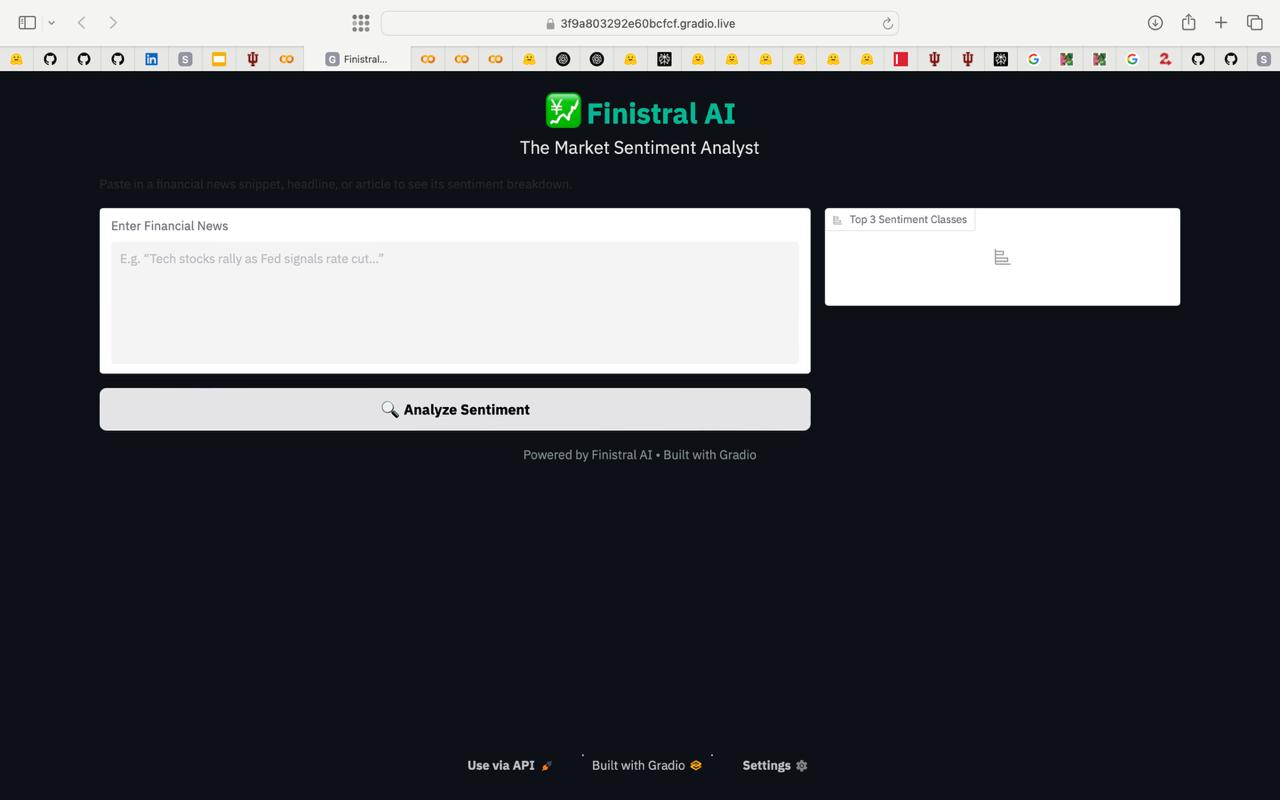
\includegraphics[width=0.75\textwidth]{figures/image1.jpeg}
\caption{Finistral-7B-LoRA Gradio interface: single-sentence query view.}
\label{fig:gui1}
\end{figure}

\begin{figure}[htbp]
\centering
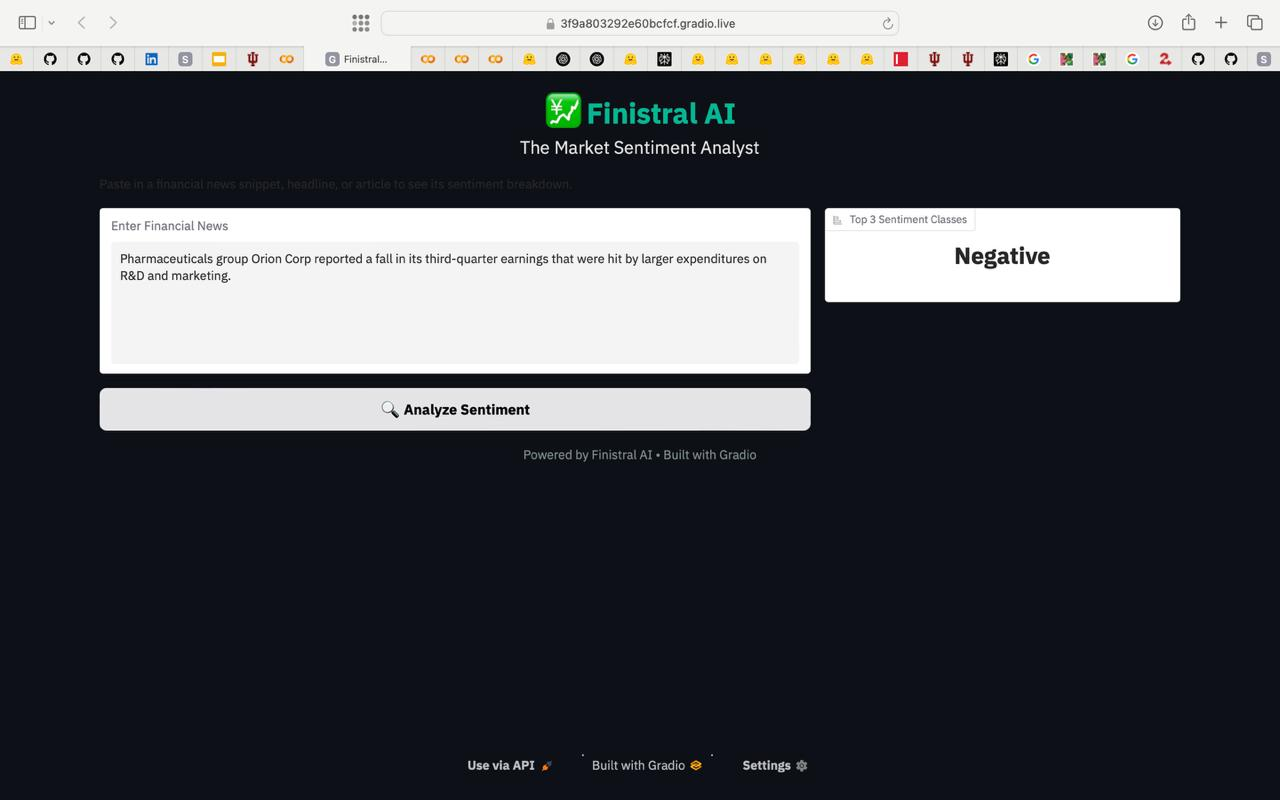
\includegraphics[width=0.75\textwidth]{figures/image2.jpeg}
\caption{Finistral-7B-LoRA Gradio interface: prediction output view.}
\label{fig:gui2}
\end{figure}


\section{Experiment}

This section describes the evaluation protocol, baselines, metrics, and implementation details we use to assess Finistral-7B-LoRA on sentence-level financial sentiment classification.

\subsection{Baselines}

In the revised evaluation, each baseline is run under its own native inference procedure (its published prompt template and the correct backbone), with left-padding for decoder-only generation, \texttt{max\_new\_tokens}-bounded greedy decoding, and a strict (non-defaulting) label parser. This corrects the original protocol, in which a \emph{single} shared Alpaca prompt, right-padding, a \texttt{max\_length}/\texttt{padding} collision, and a neutral-defaulting parser were applied uniformly to every model. These defects drove several baselines below their majority-class floor (Section~\ref{sec:contamination}).

\begin{table}[htbp]
\centering
\caption{Baselines}
\label{tab:baselines}
\begin{tabular}{clcc}
\toprule
\textbf{ID} & \textbf{Model} & \textbf{Adapter params (config)} & \textbf{Fine-tuned?} \\
\midrule
B\textsubscript{1} & Mistral-7B-v0.1 (zero-shot)  & n/a (base 7.24\,B) & $\times$ \\
B\textsubscript{2} & FinGPT-mt-Llama2-7B-LoRA  & 6.29\,M ($r{=}8$, q/k/v) & $\checkmark$ \\
B\textsubscript{3} & FinGPT-Llama-3-8B-LoRA    & 3.41\,M ($r{=}8$, q/v) & $\checkmark$ \\
B\textsubscript{4} & FinGPT-Falcon-7B-LoRA     & 2.36\,M ($r{=}8$, fused QKV) & $\checkmark$ \\
B\textsubscript{5} & FinGPT-Bloom-7B1-LoRA     & 3.93\,M ($r{=}8$, fused QKV) & $\checkmark$ \\
B\textsubscript{6} & FinBERT (ProsusAI)        & 110\,M (full fine-tune) & $\checkmark$ \\
\bottomrule
\end{tabular}
\par\smallskip
{\footnotesize Adapter parameter counts are read from each adapter's published \texttt{adapter\_config.json} and verified against its weight-file size (our original submission's uniform ``9\,M'' figures were incorrect). FinBERT is an encoder classifier evaluated through its classification head rather than by generation; note that FinBERT's own fine-tuning data includes Financial PhraseBank, so its FPB scores carry an analogous train/test caveat and the external datasets provide its fair comparison.}
\end{table}

\subsection{Metrics}

\textbf{Accuracy:} fraction of correct predictions.

\textbf{Weighted F1:} F1 averaged with class-frequency weights; it tracks performance on the label mix actually encountered in each dataset. Because it down-weights rare classes, we additionally report macro F1 (the imbalance-sensitive view, unweighted over classes) for every comparison in Appendix~A.

\textbf{Significance:} every pairwise comparison against Finistral carries a per-example McNemar test (exact binomial when discordant pairs $b{+}c<25$, continuity-corrected $\chi^2$ otherwise) and a paired percentile-bootstrap 95\,\% confidence interval (10{,}000 resamples) on the accuracy difference.

\subsection{Main Result}

We report two distinct quantities and are careful not to conflate them. Table~\ref{tab:test-results} reproduces the \emph{original, contaminated} in-distribution numbers (full \texttt{sentences\_allagree} split, original harness); these are retained only as a contamination diagnostic. Table~\ref{tab:corrected-results} reports the \emph{corrected} numbers: Finistral evaluated on the 560-sentence decontaminated remainder and on external datasets, with all baselines re-run under their native inference procedures. The original ``+78 F1 over the strongest FinGPT baseline'' claim conflated a contamination-inflated model with harness-deflated baselines and is withdrawn.

\begin{table}[htbp]
\centering
\caption{Original (contaminated) in-distribution results on the full \texttt{sentences\_allagree} split, original harness. Retained only as a contamination diagnostic; 75.2\,\% of these sentences were seen in training (Section~\ref{sec:contamination}). The baseline scores below the 61.6\,\% majority-class floor are harness artifacts, \emph{not} measures of model quality.}
\label{tab:test-results}
\begin{tabular}{lcc}
\toprule
\textbf{Model} & \textbf{Accuracy} & \textbf{Weighted F1} \\
\midrule
\textbf{Finistral-7B-LoRA (ours, \emph{contaminated})} & \textbf{0.9956} & \textbf{0.9956} \\
Mistral-7B-Base \emph{(broken harness)}                    & 0.4125          & 0.2967 \\
FinGPT-mt-Llama2-7B-LoRA \emph{(broken harness)}          & 0.1564          & 0.0789 \\
FinGPT-Llama-3-8B-LoRA \emph{(broken harness)}            & 0.2310          & 0.2112 \\
FinGPT-Falcon-7B-LoRA \emph{(broken harness)}             & 0.2102          & 0.1713 \\
FinGPT-Bloom-7B1-LoRA \emph{(broken harness)}             & 0.1312          & 0.0310 \\
\bottomrule
\end{tabular}
\end{table}

\begin{table}[htbp]
\centering
\caption{Corrected results on the exact-match-decontaminated evaluation sets under the fixed harness (\texttt{eval\_harness\_fixed.py} + \texttt{stats\_report.py}): the decontaminated 560-sentence FPB remainder, FiQA-SA (all splits pooled then row-wise decontaminated against the FinGPT corpus, $n{=}235$), and Twitter Financial News Sentiment (validation split, row-wise decontaminated, $n{=}2{,}373$). Decoding is greedy and deterministic (single pass; identical outputs across seeds by construction). \textbf{Bold} marks the best value per column. Complete statistics (macro F1, unparseable rates, McNemar $p$-values, and bootstrap confidence intervals for every comparison) are in Appendix~A; all comparisons are conditional on each model's native prompt template (Section~\ref{sec:contamination} and the ablation show template choice alone can shift accuracy by 9--10 points).}
\label{tab:corrected-results}
\begin{tabular}{lcccccc}
\toprule
 & \multicolumn{2}{c}{\textbf{FPB-560}} & \multicolumn{2}{c}{\textbf{FiQA-SA}} & \multicolumn{2}{c}{\textbf{TFNS}} \\
\cmidrule(lr){2-3}\cmidrule(lr){4-5}\cmidrule(lr){6-7}
\textbf{Model} & \textbf{Acc} & \textbf{wF1} & \textbf{Acc} & \textbf{wF1} & \textbf{Acc} & \textbf{wF1} \\
\midrule
\textbf{Finistral-7B-LoRA (ours)} & \textbf{0.9893} & \textbf{0.9893} & \textbf{0.8766} & \textbf{0.8833} & \textbf{0.7893} & 0.7959 \\
Mistral-7B-v0.1 (zero-shot)       & 0.0036 & 0.0070 & 0.0128 & 0.0252 & 0.0013 & 0.0025 \\
FinGPT-mt-Llama2-7B-LoRA          & 0.9857 & 0.9857 & 0.8085 & 0.8301 & 0.7644 & 0.7713 \\
FinGPT-Llama-3-8B-LoRA            & 0.9339 & 0.9410 & 0.6213 & 0.7219 & 0.7804 & \textbf{0.8211} \\
FinGPT-Falcon-7B-LoRA             & 0.9696 & 0.9697 & 0.8553 & 0.8594 & 0.7307 & 0.7377 \\
FinGPT-Bloom-7B1-LoRA             & 0.8946 & 0.8934 & 0.6936 & 0.6914 & 0.6827 & 0.6986 \\
FinBERT (ProsusAI)                & 0.9643 & 0.9648 & 0.5149 & 0.6147 & 0.7252 & 0.7329 \\
\bottomrule
\end{tabular}
\end{table}

On the contaminated split only ten of 2,264 samples are misclassified, a direct consequence of the model having seen three-quarters of the split during training. The genuine error profile is characterised on the decontaminated and external sets in Section~\ref{sec:contamination}.

\subsection{Hardware \& Software}

\textbf{Training environment:} $2 \times$ NVIDIA A100 40\,GB on Indiana University's Big Red 200; PyTorch 2.2, Transformers 4.39, PEFT 0.10; \texttt{bfloat16} throughout, no quantisation.

\textbf{Corrected evaluation environment:} $1 \times$ NVIDIA A100 40\,GB (Big Red 200); PyTorch 2.4.1, Transformers 4.44.2, PEFT 0.11.1, Accelerate 0.33.0, Datasets 2.20.0. Generation is greedy (\texttt{do\_sample=False}, \texttt{num\_beams=1}) with \texttt{max\_new\_tokens=8}, left-padded batches, and per-model native prompt templates; the label parser matches whole words on the decoded continuation only and reports unparseable outputs separately instead of defaulting them to neutral.

\subsection{Data Contamination Analysis}
\label{sec:contamination}

We audited the overlap between our training corpus, \texttt{FinGPT/fingpt-sentiment-train} (76{,}772 sentences), and our evaluation set, Financial PhraseBank \texttt{sentences\_allagree} (2{,}264 lines; 2{,}259 unique). Financial PhraseBank is one of the four constituent sources aggregated into the FinGPT sentiment corpus (alongside FiQA-SA, Twitter Financial News Sentiment, and News-With-GPT-Instructions), so overlap is expected by construction. We measured it directly.

\textbf{Procedure.} We normalise both corpora (lowercasing, Unicode NFKC folding, punctuation stripping, whitespace collapse, which is essential because Financial PhraseBank uses spaced punctuation such as ``\texttt{USD 2.3 mn .}'') and test each evaluation sentence for (a) exact and (b) normalised membership in the training inputs, recording the training-side gold label for every match. The full script is released as \texttt{leakage\_analysis.py} / \texttt{measure\_leakage\_local.py}.

\textbf{Findings.} The overlap is severe and is summarised in Table~\ref{tab:contamination}: \textbf{1{,}699 of the 2{,}259 unique evaluation sentences (75.2\,\%) appear verbatim in the training inputs, and in 100\,\% of those matches the training-side gold label is identical to the Financial PhraseBank label}, uniformly across classes. Reproducing the training script's own \texttt{train\_test\_split(test\_size=0.05, seed=42)}, $\approx$\,1{,}614 of these leaked sentences fall in the 95\,\% fine-tuning partition. The model was therefore scored on the exact (sentence, label) pairs it was trained on, which fully accounts for the 99.56\,\% headline accuracy.

\begin{table}[htbp]
\centering
\caption{Train/test overlap between \texttt{FinGPT/fingpt-sentiment-train} and Financial PhraseBank \texttt{sentences\_allagree} (locally reproduced).}
\label{tab:contamination}
\begin{tabular}{lc}
\toprule
\textbf{Quantity} & \textbf{Value} \\
\midrule
Unique evaluation sentences            & 2{,}259 \\
Verbatim (exact) overlap with training & 1{,}699 (75.2\,\%) \\
Normalised overlap with training       & 1{,}699 (75.2\,\%) \\
Label agreement among matched          & 1{,}699 / 1{,}699 (100\,\%) \\
Decontaminated remainder (unseen)      & 560 (24.8\,\%) \\
\bottomrule
\end{tabular}
\end{table}

\textbf{Near-duplicate audit.} Exact and normalised matching cannot catch paraphrases or lightly edited variants, so we additionally computed, for every retained evaluation sentence, its maximum token-set Jaccard similarity against all 30{,}209 unique normalised training inputs (inverted-index blocked; released as \texttt{near\_duplicate\_audit.py}). The near-duplicate tail is small but nonzero: on FPB-560, 22 sentences (3.9\,\%) have $J \ge 0.7$, 10 (1.8\,\%) $J \ge 0.8$, and 3 (0.5\,\%) $J \ge 0.9$; on FiQA-SA, 5 (2.1\,\%) reach $J \ge 0.7$ and none $J \ge 0.9$; on TFNS, 119 (5.0\,\%) reach $J \ge 0.7$ and 15 (0.6\,\%) $J \ge 0.9$. Even under the worst-case assumption that every $J \ge 0.7$ sentence is answered by memorisation, Finistral's FPB-560 accuracy changes by at most 3.9 points, so near-duplicate leakage cannot account for the corrected results. We accordingly describe our sets as \emph{exact-match-decontaminated} rather than leakage-free, and release the audit alongside the data.

\textbf{Decontamination and corrected evaluation.} We remove every leaked sentence and retain the \textbf{560-sentence disjoint remainder} (neutral 353, positive 130, negative 77) as an exact-match-decontaminated Financial PhraseBank test set (released as \texttt{fpb\_decontaminated.csv}). Because even this remainder shares Financial PhraseBank's stylistic distribution, we additionally evaluate on external sets, decontaminated \emph{row-wise} against the FinGPT training inputs under the same normalisation: \textbf{FiQA-SA} (all splits pooled, then leaked rows removed, $n{=}235$; pooling is necessary because FiQA is itself a FinGPT constituent and its test split alone is 78\,\% contaminated) and the \textbf{Twitter Financial News Sentiment} validation split ($n{=}2{,}373$ after removing 15 leaked/duplicate rows). Dataset provenance, label mappings, and dropped-row counts are released in \texttt{data\_eval/PROVENANCE.md}. Corrected numbers, with per-example McNemar tests and paired-bootstrap 95\,\% confidence intervals against every baseline, are reported in Table~\ref{tab:corrected-results}.

\textbf{Harness defects underlying the baselines.} Independently of contamination, the original baseline scores (13--23\,\%, below the 61.6\,\% majority-class floor) are artifacts of the evaluation harness, not of the models. The committed notebook logs contain hundreds of \texttt{padding\_side=right} warnings for decoder-only models; generation was called as \texttt{generate(**tok, max\_length=512)} with \texttt{padding=True} (so \texttt{max\_length} is ignored and generations ramble); a single Alpaca prompt was applied to every model rather than each adapter's native template; a quantisation config built from invalid \texttt{BitsAndBytesConfig} keyword arguments silently degraded to plain int8; and the label parser defaulted unmatched outputs to ``neutral.'' The corrected harness (\texttt{eval\_harness\_fixed.py}) fixes each of these and reports per-baseline confusion matrices.

\section{Result Analysis \& Discussion}

\subsection{Quantitative Gains}

The large apparent margins reported in our original submission ($+69$ F1 over zero-shot Mistral-7B; $+78$--$96$ F1 over the FinGPT LoRA baselines; $+3$--$6$ accuracy points over FinBERT) do not survive scrutiny and are withdrawn. As Section~\ref{sec:contamination} establishes, the Finistral side of every such comparison was inflated by 75.2\,\% train/test overlap, while the FinGPT baselines were deflated below their majority-class floor by harness defects. The near-perfect per-class F1 on the contaminated split (Negative 98.7\,\%, Neutral 99.4\,\%, Positive 99.3\,\%) and the reduction of errors to ``10 of 2{,}264'' are likewise consequences of memorisation, not generalisation, and the confusion matrix in Figure~\ref{fig:confusion} should be read as a diagnostic of contamination rather than of model quality. The honest performance picture is given by the decontaminated and external evaluations in Table~\ref{tab:corrected-results}. On the decontaminated FPB remainder, Finistral attains 98.93\,\% accuracy with per-class F1 of 0.974 (negative), 0.993 (neutral), and 0.989 (positive), but this is \emph{not} a statistically significant advantage over the strongest baseline (FinGPT-mt-Llama2, 98.57\,\%; McNemar $p = 0.77$), and both models plausibly benefit from FPB's narrow stylistic distribution even after sentence-level decontamination. The external sets are more informative. On FiQA-SA, Finistral leads on accuracy and weighted F1 (87.66\,\% / 0.8833), significantly above FinGPT-mt-Llama2 ($p = 0.012$, unadjusted), FinGPT-Llama-3 ($p = 7.2\times10^{-11}$), and FinBERT ($p = 3.1\times10^{-17}$), though not above FinGPT-Falcon (85.53\,\%, $p = 0.42$); on macro F1, however, Finistral (0.700) \emph{trails} FinGPT-Falcon (0.723), reflecting weakness on FiQA's tiny neutral class (F1 0.276 on 12 examples). Appendix~A reports macro F1 for every comparison. On TFNS, Finistral (78.93\,\%) is statistically tied with the strongest baseline, FinGPT-Llama-3 (78.04\,\%, $p = 0.41$), and significantly above the remaining adapters and FinBERT (mt-Llama2 $p = 2.1\times10^{-3}$; Falcon, Bloom, and FinBERT all $p < 10^{-8}$). The zero-shot Mistral-7B backbone emits almost no parseable label under strict parsing (99\,\% unparseable outputs): fine-tuning confers, at minimum, output-format compliance and, given the fine-tuned models' accuracy, task competence with it. All $p$-values are unadjusted across the 21 pairwise tests (Appendix~A states which conclusions survive a Holm--Bonferroni correction); notably, \emph{no comparison against the strongest per-dataset baseline reaches significance} (FPB-560 $p=0.77$; FiQA-SA vs Falcon $p=0.42$; TFNS vs Llama-3 $p=0.41$). In sum: the corrected evaluation shows Finistral statistically indistinguishable from the best FinGPT-class adapter on each dataset, significantly better than several others, and clearly ahead of FinBERT off-distribution, not the categorical superiority the original submission asserted.

\begin{figure}[htbp]
\centering
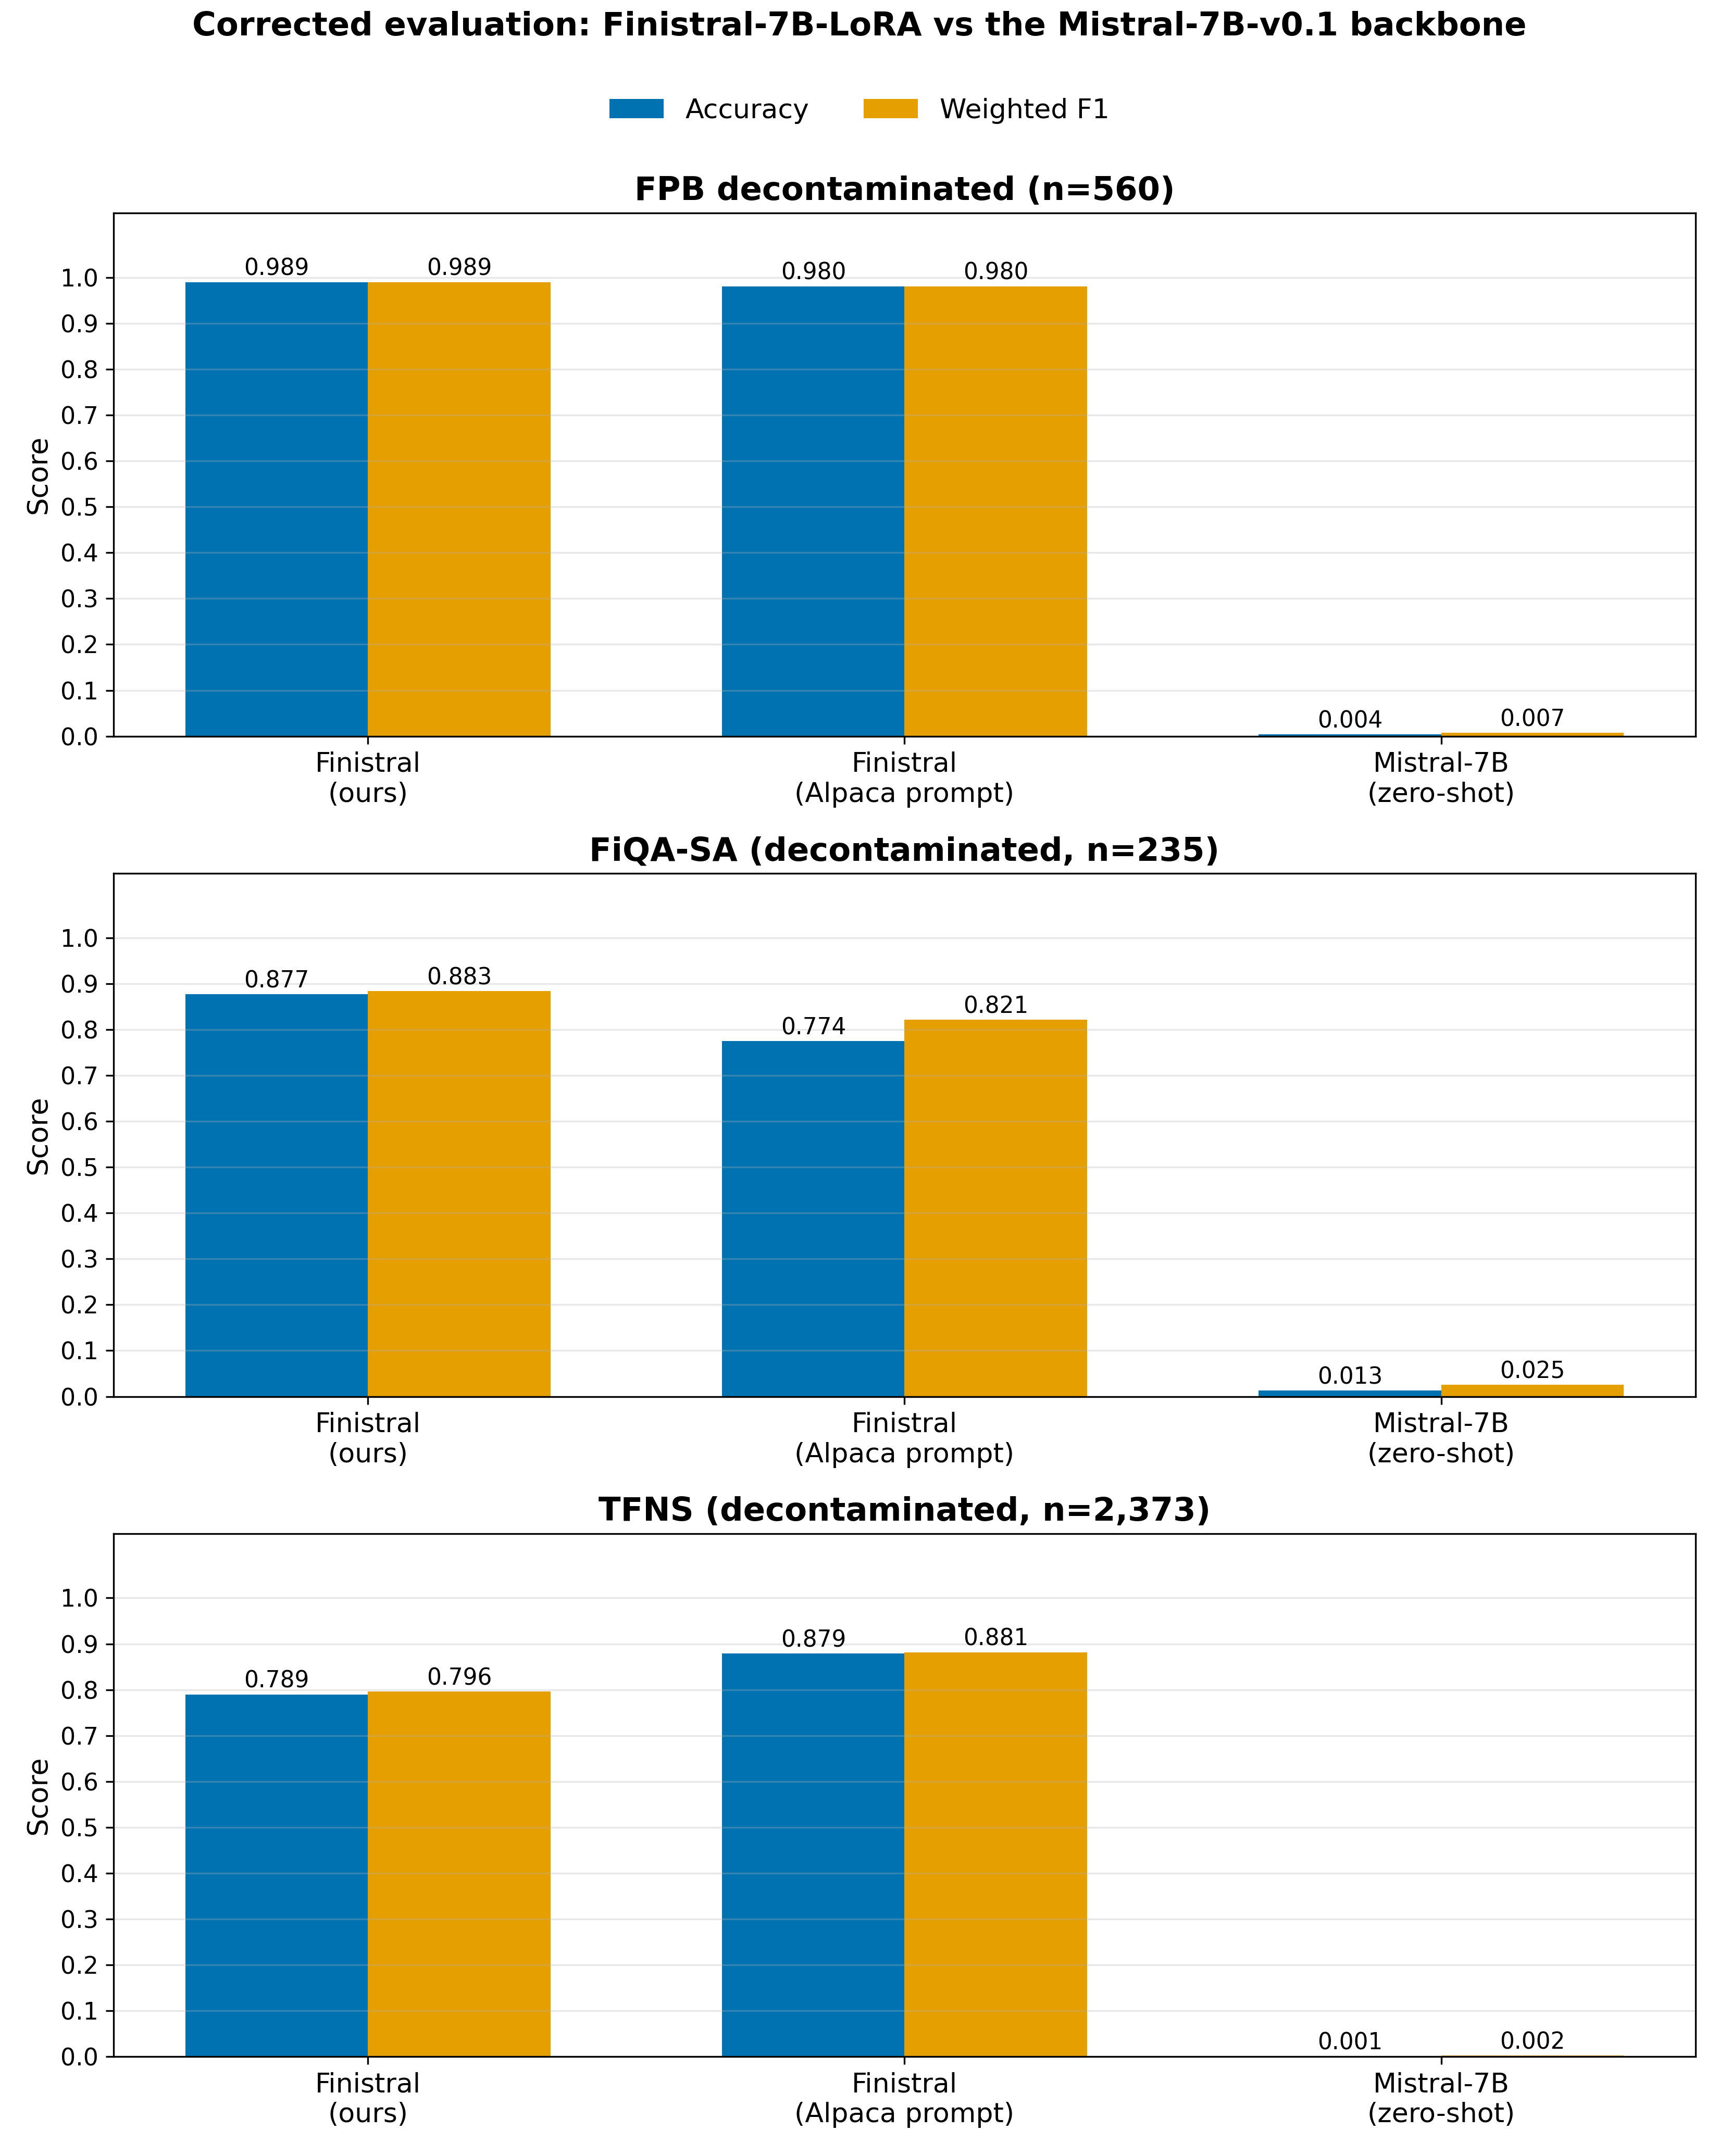
\includegraphics[width=\textwidth]{figures/image3_corrected.png}
\caption{Corrected comparison on the exact-match-decontaminated sets: Finistral-7B-LoRA (training template and Alpaca-template ablation) vs the Mistral-7B-v0.1 zero-shot backbone on the decontaminated FPB-560, FiQA-SA ($n{=}235$), and TFNS ($n{=}2{,}373$) sets.}
\label{fig:bar-comparison}
\end{figure}

\begin{figure}[htbp]
\centering
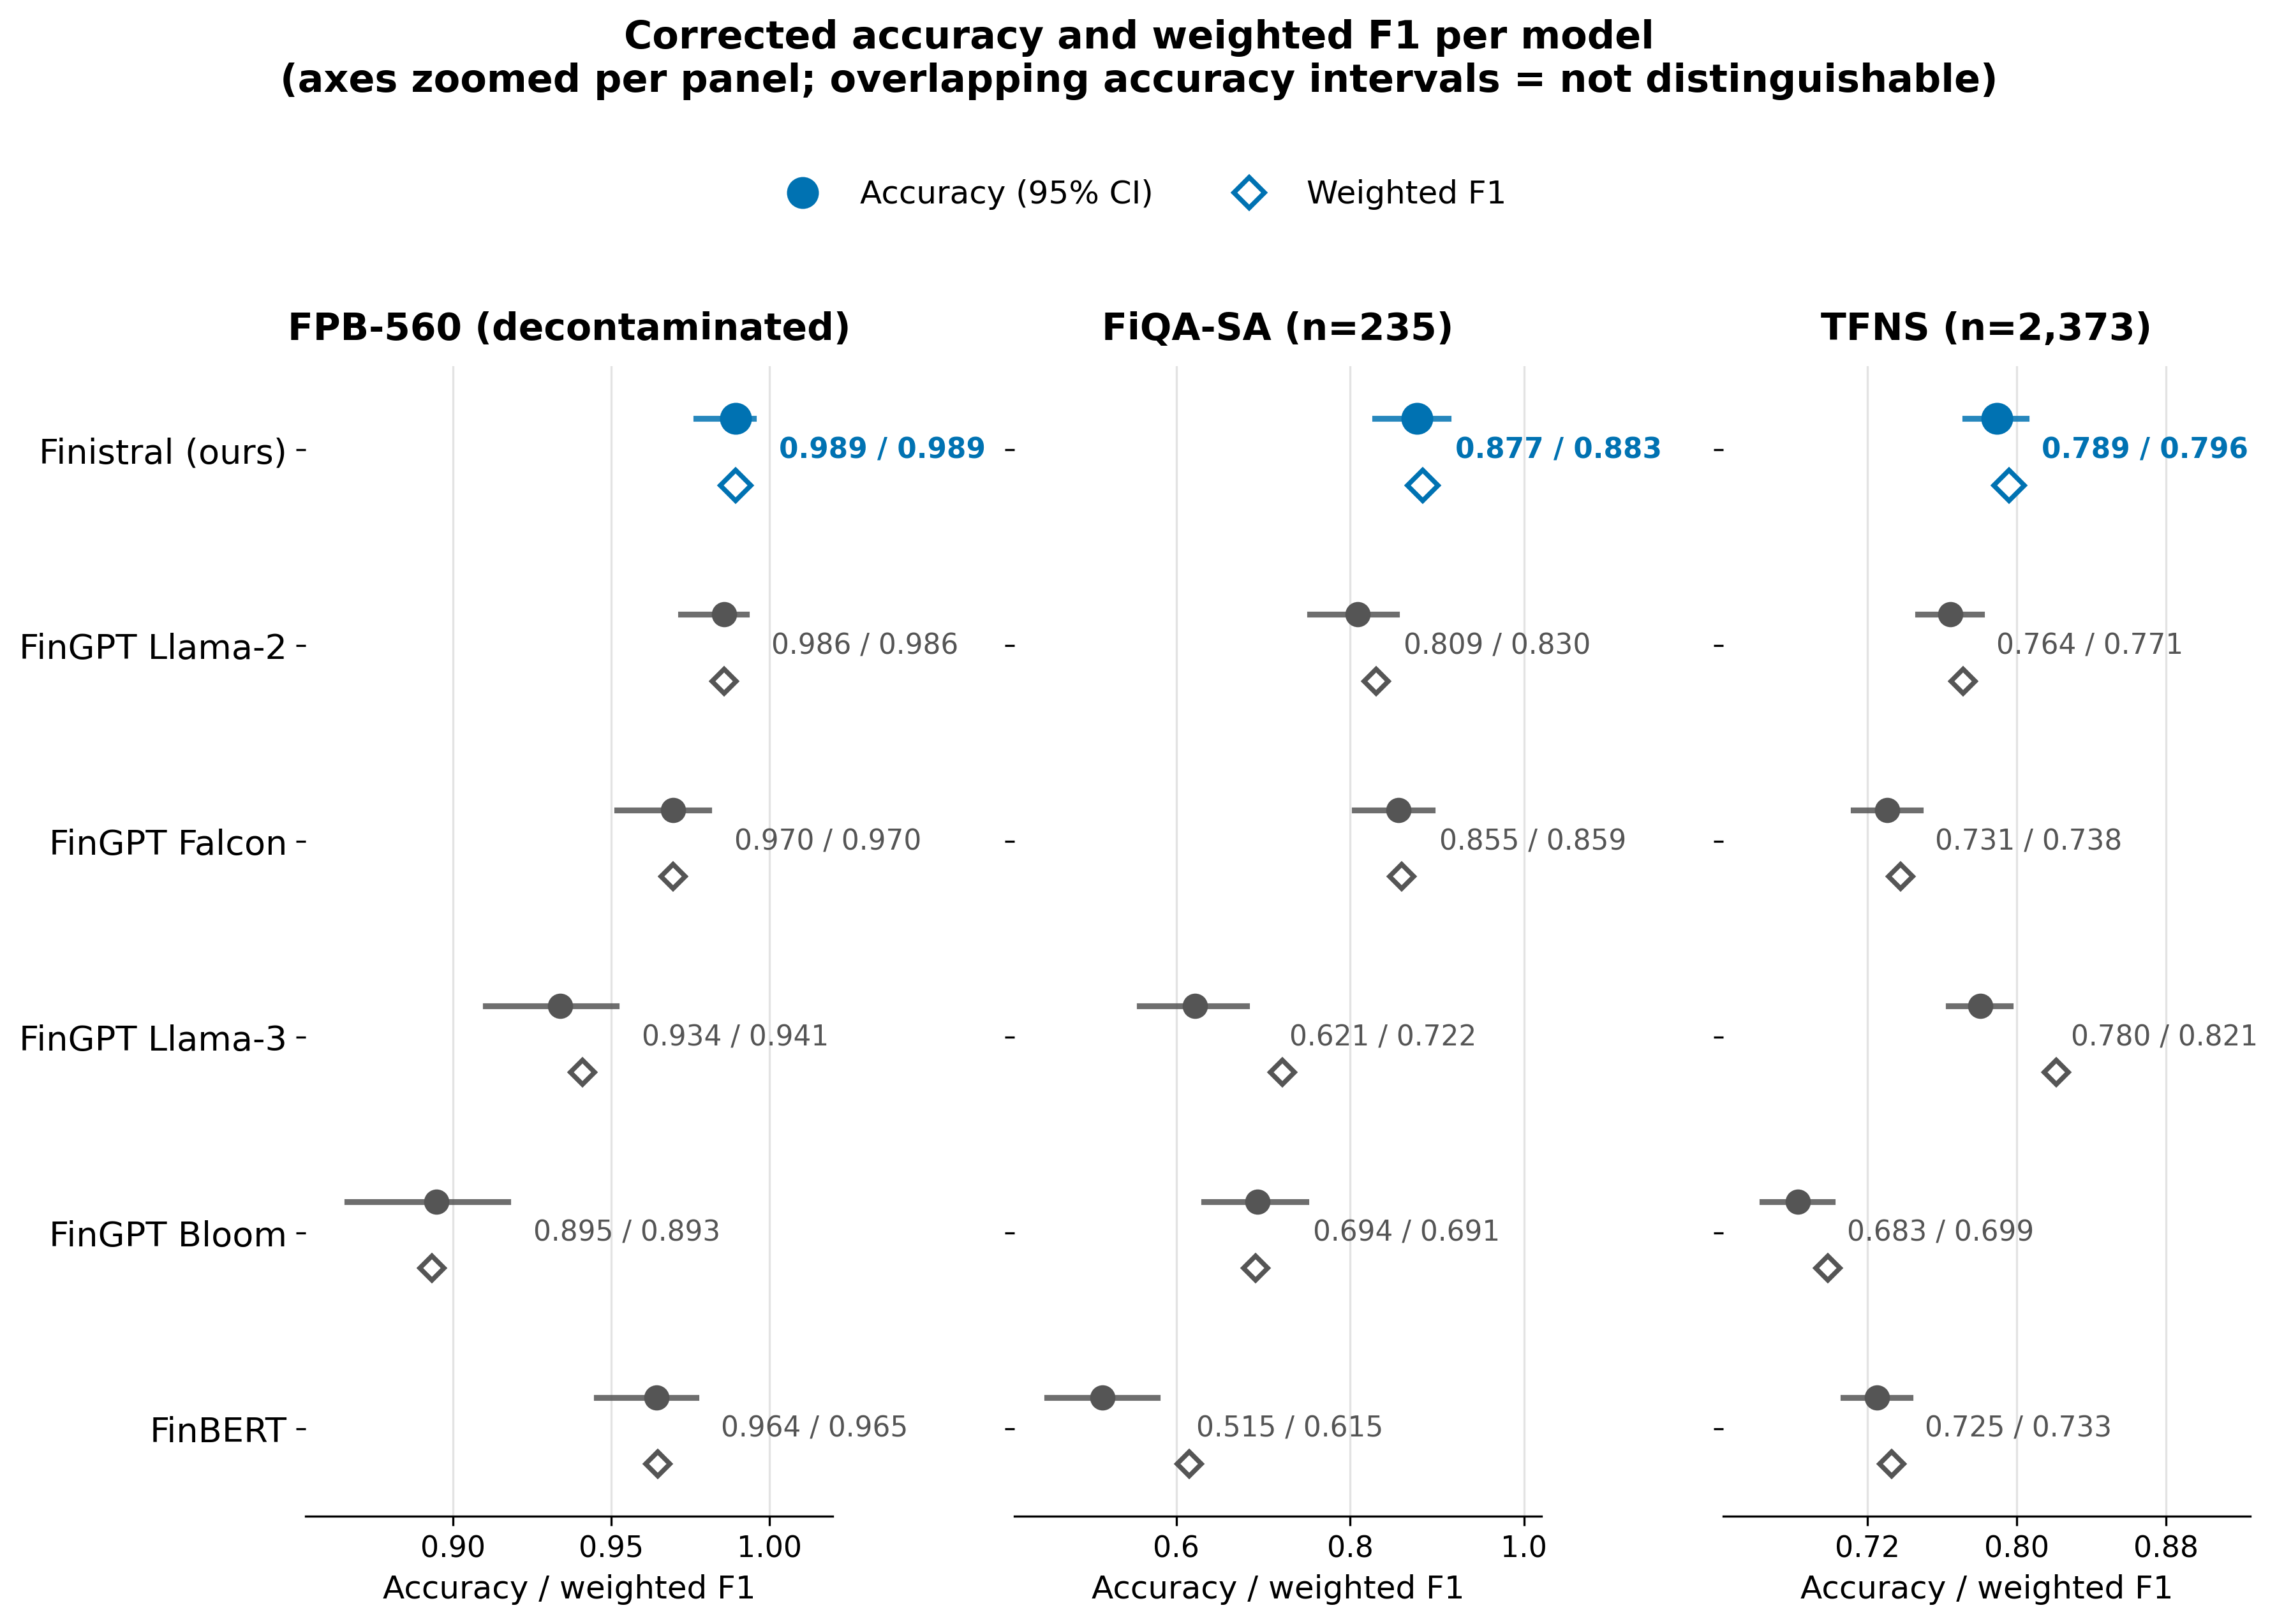
\includegraphics[width=\textwidth]{figures/dotplot_comparison.png}
\caption{Corrected accuracy (filled circles, with 95\,\% Wilson confidence intervals) and weighted F1 (open diamonds) for Finistral-7B-LoRA against all FinGPT adapter baselines and FinBERT on the exact-match-decontaminated sets; numeric labels give accuracy\,/\,weighted F1. Axes are zoomed per panel to resolve small differences; because value is encoded by position rather than bar length, the non-zero origin introduces no visual exaggeration. Overlapping accuracy intervals indicate differences that are not statistically distinguishable. Note the overlap with FinGPT-mt-Llama2 on FPB-560, FinGPT-Falcon on FiQA-SA, and FinGPT-Llama-3 on TFNS, matching the McNemar results in Appendix~A. The two metrics do not always agree: on TFNS, FinGPT-Llama-3 attains a higher weighted F1 (0.821) than Finistral (0.796) despite lower accuracy, and on FiQA-SA FinGPT-Falcon leads on macro F1 (Appendix~A). The unparseable-dominated zero-shot backbone is omitted here and shown in Figure~\ref{fig:bar-comparison}.}
\label{fig:fingpt-comparison}
\end{figure}

\begin{figure}[htbp]
\centering
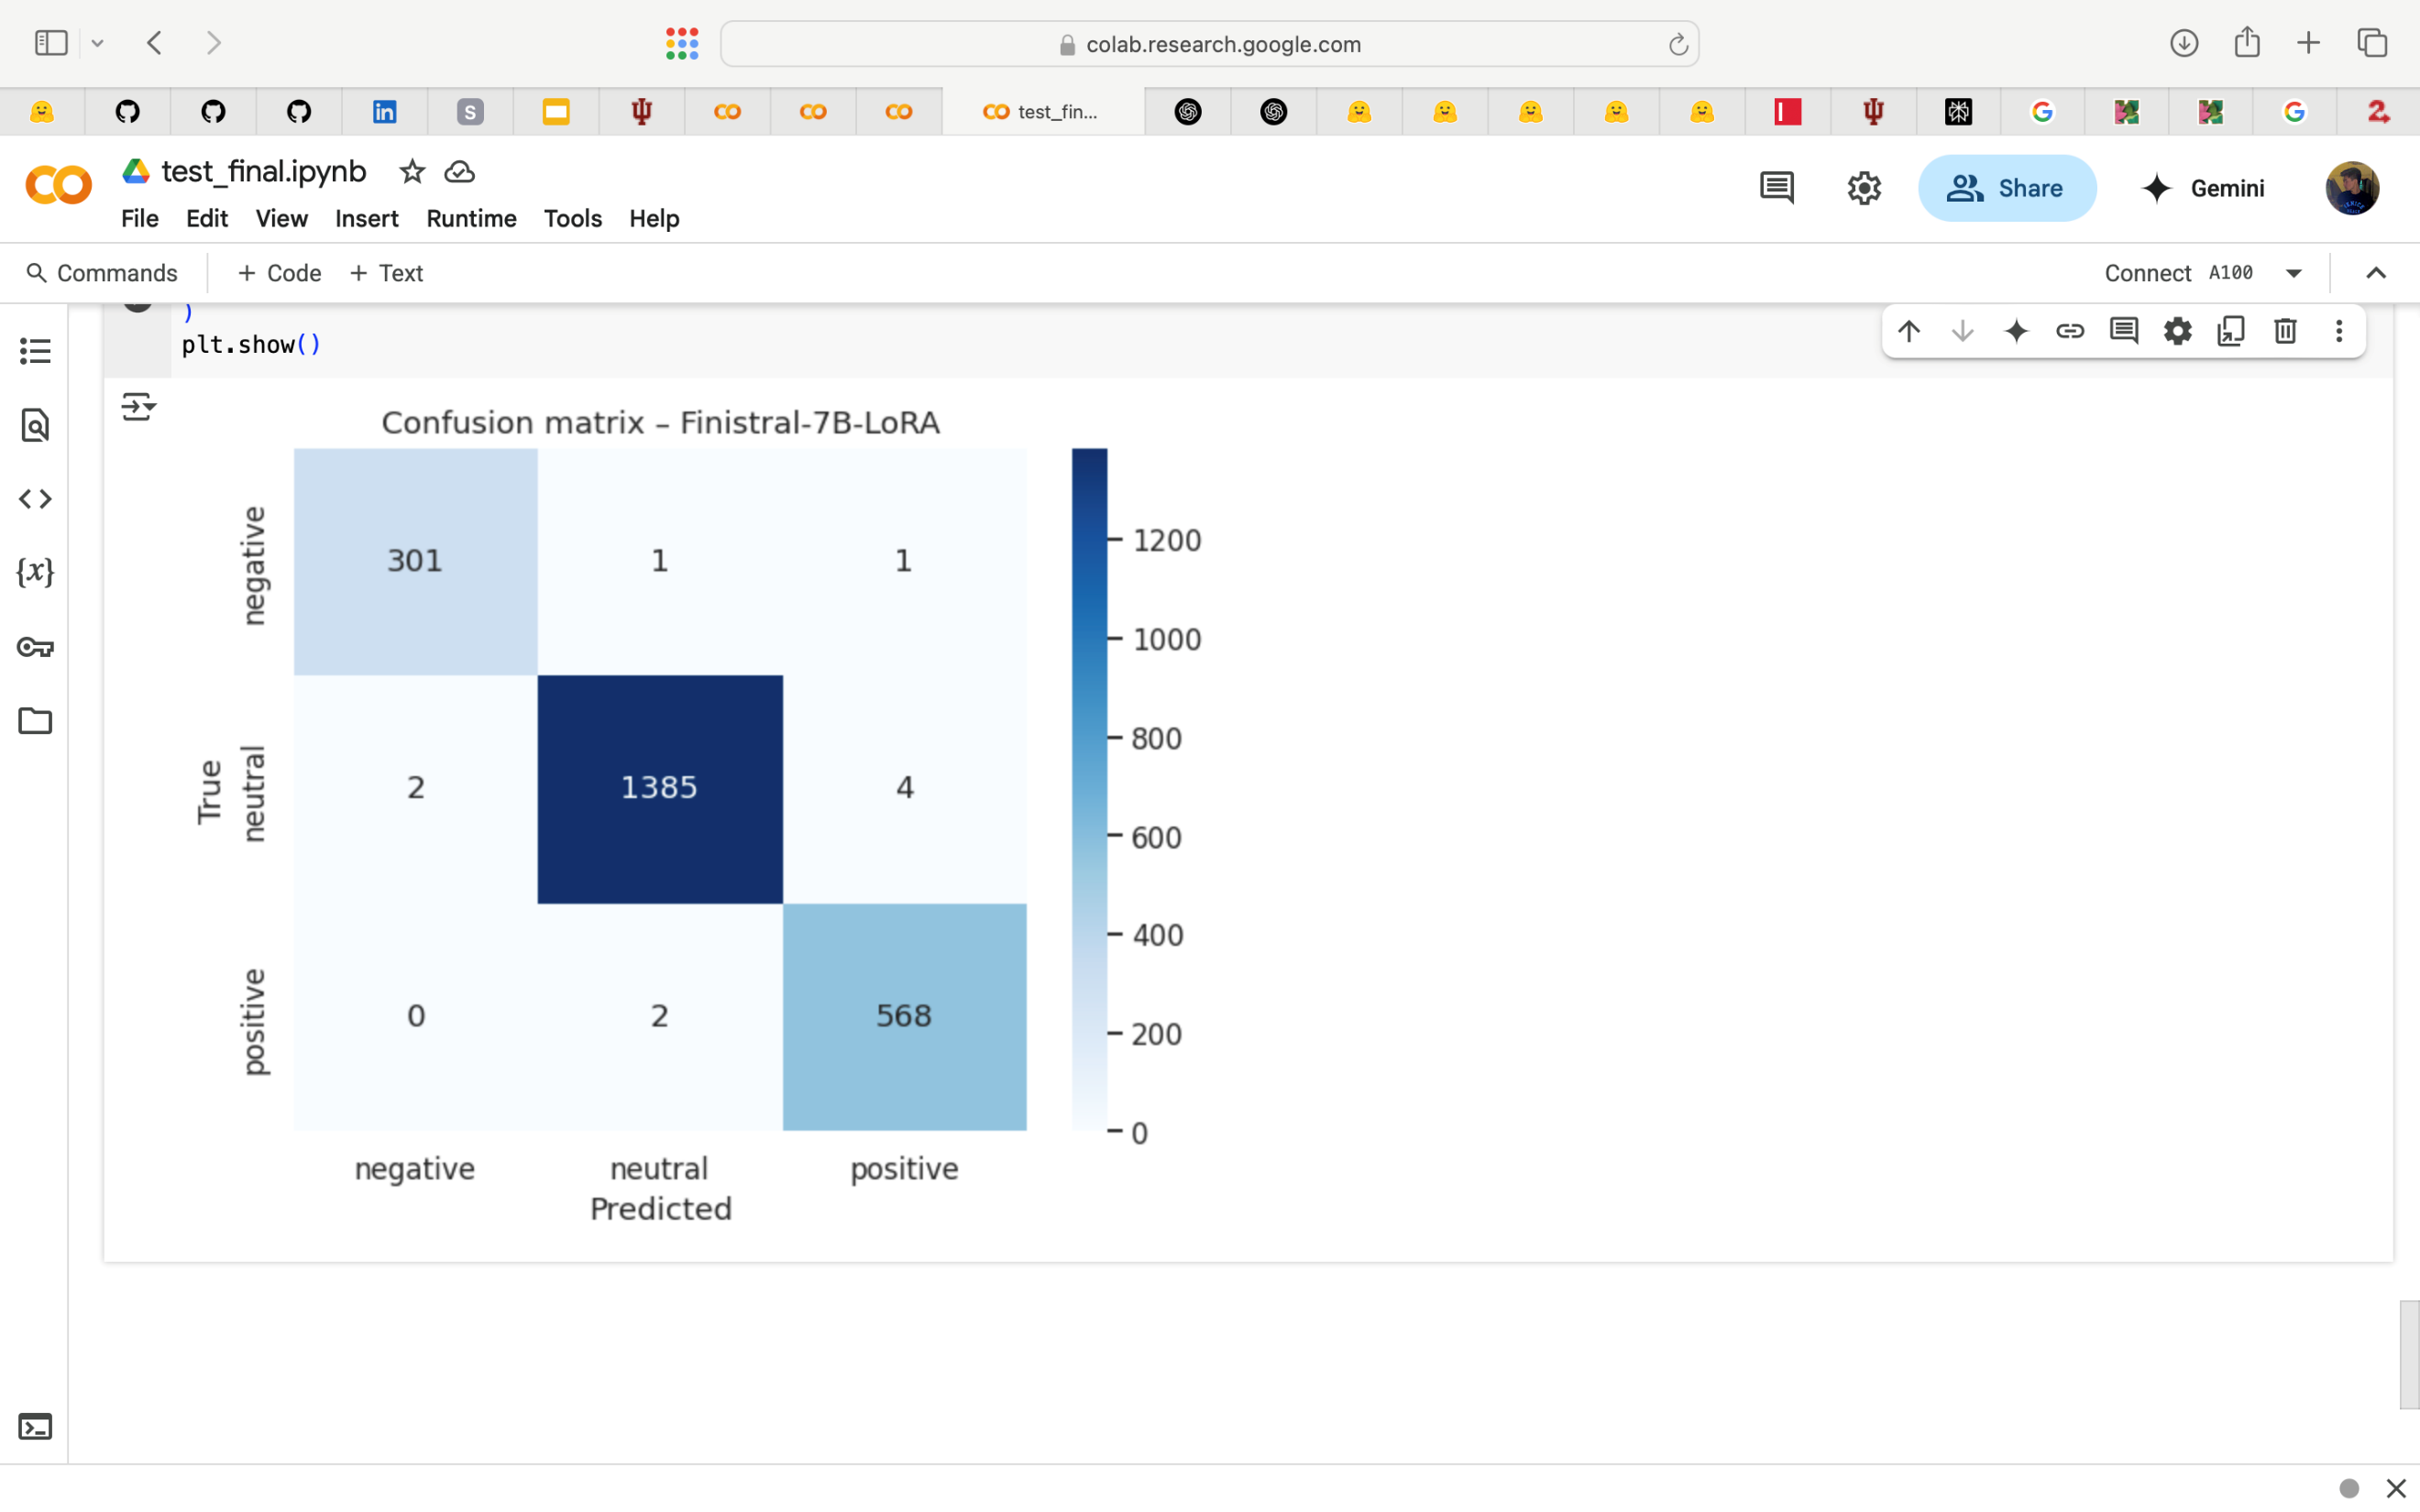
\includegraphics[width=0.52\textwidth]{figures/image5.png}
\caption{Confusion matrix of Finistral-7B-LoRA on the \emph{original, contaminated} full split, retained solely as a contamination diagnostic (Section~\ref{sec:contamination}); the corrected per-model confusion matrices appear in Figure~\ref{fig:confusion-grid}.}
\label{fig:confusion}
\end{figure}

\begin{figure}[p]
\centering
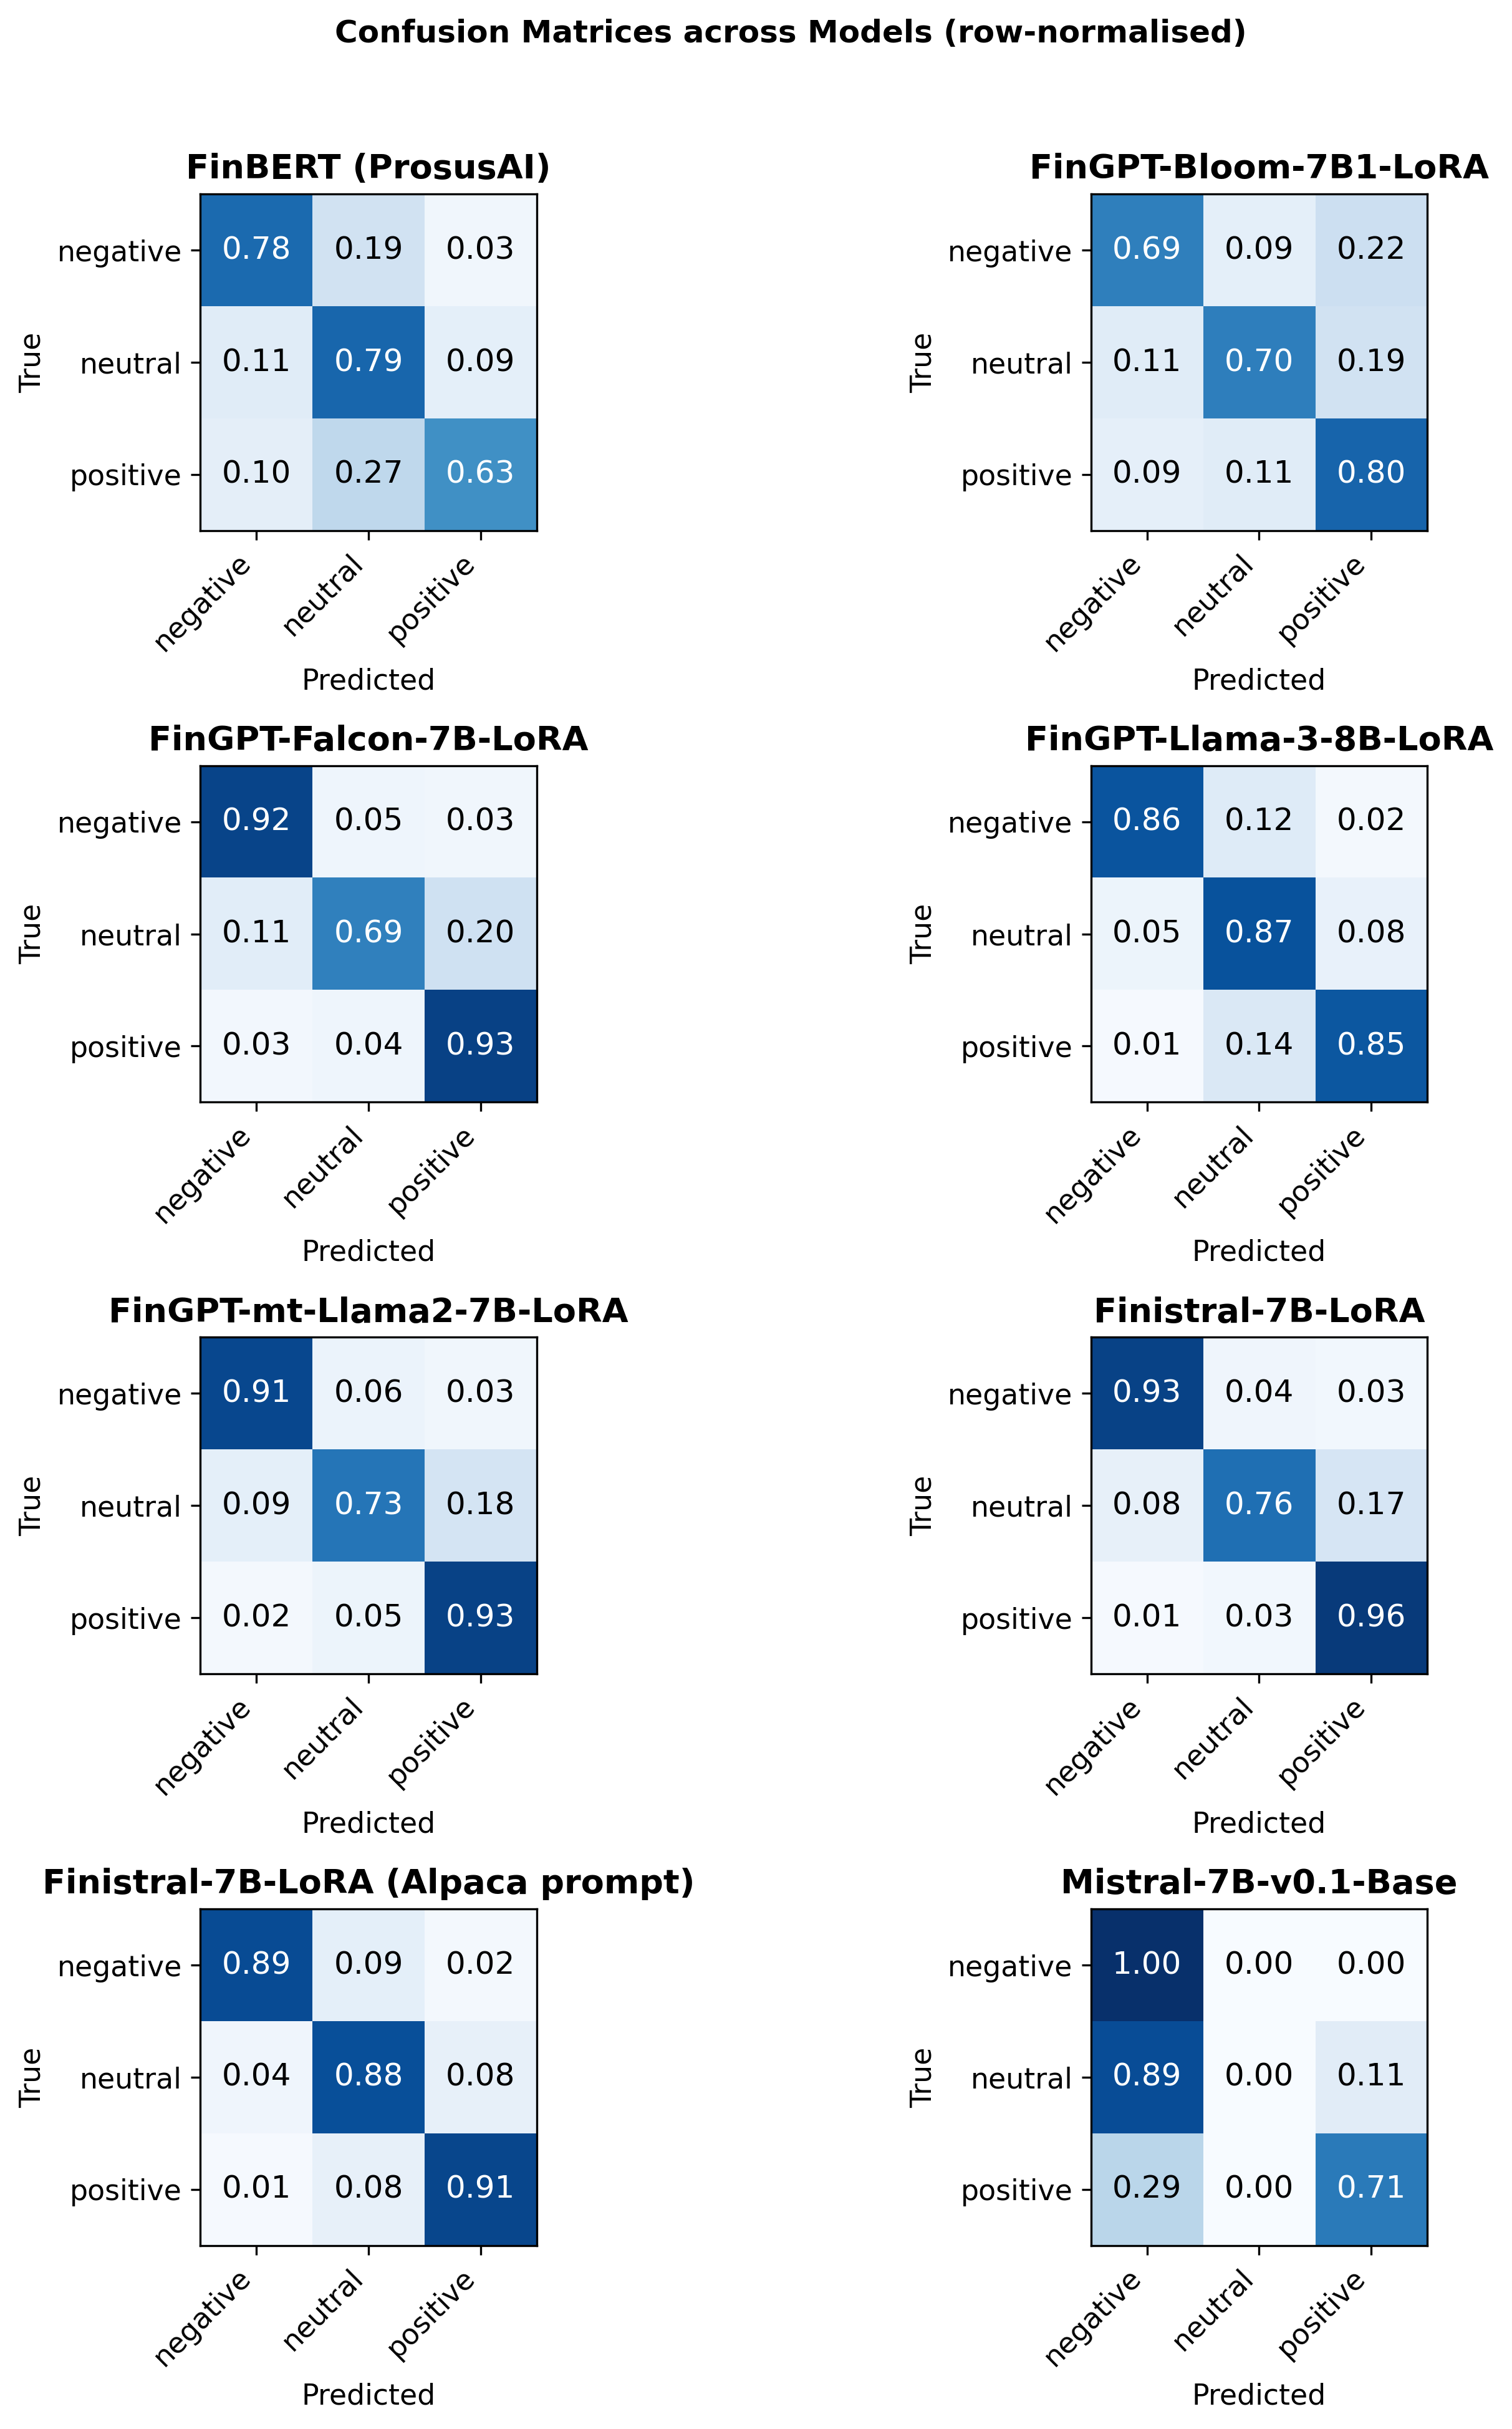
\includegraphics[height=0.9\textheight,keepaspectratio]{figures_corrected/confusion_matrix_grid_normalized_page.png}
\caption{Row-normalised confusion matrices for every evaluated model under the corrected protocol on the exact-match-decontaminated sets (all three pooled; per-dataset and raw-count variants are released with the code). The \emph{unparseable} column shows strict-parser failures, dominant only for the zero-shot backbone.}
\label{fig:confusion-grid}
\end{figure}

\subsection{Training Dynamics Insight}

Validation loss reached its minimum (0.1009) at epoch 2 and then rose, a classic sign of incipient overfitting. Selecting the epoch-2 checkpoint therefore maximises generalisation.

\subsection{Efficiency vs.\ Quality Tradeoffs}

\begin{table}[htbp]
\centering
\caption{Efficiency vs.\ Quality Tradeoffs}
\label{tab:efficiency}
\begin{tabular}{lcc}
\toprule
\textbf{Dimension} & \textbf{Finistral-7B-LoRA} & \textbf{Best FinGPT adapter} \\
\midrule
Trainable params  & 41.94\,M ($r{=}16$, all-linear) & 2.4--6.3\,M ($r{=}8$) \\
Adapter size      & 83.9\,MB (fp16)  & 5--14\,MB \\
Train time ($2\times$A100) & $\approx$ 120\,min & (published adapters) \\
Weighted F1 (FPB-560 / FiQA / TFNS) & 0.989 / 0.883 / 0.796 & 0.986 / 0.859 / 0.821$^{\dagger}$ \\
\bottomrule
\end{tabular}
\par\smallskip
{\footnotesize $^{\dagger}$Best FinGPT adapter \emph{per dataset}: FinGPT-mt-Llama2 on FPB-560, FinGPT-Falcon on FiQA-SA, FinGPT-Llama-3 on TFNS.}
\end{table}

The original version of this table juxtaposed Finistral's contaminated 0.996 F1 against a FinGPT baseline's harness-broken 0.211 F1; both numbers were invalid for comparison and have been replaced with corrected figures from the exact-match-decontaminated evaluation. Two honest observations follow. First, the efficiency columns (parameter count, adapter size, train time) are unaffected by contamination and are absolute virtues of the recipe: a competitive financial-sentiment adapter for well under one GPU-day, on academic infrastructure, end-to-end reproducible. Second, however, Finistral is \emph{not} the most parameter-efficient model in its own comparison: FinGPT-mt-Llama2 trains $6.7\times$ fewer parameters (6.29\,M vs 41.94\,M) yet is statistically indistinguishable from Finistral on FPB-560 ($p=0.77$) and competitive on TFNS, with Finistral's clearest win confined to FiQA-SA. The defensible claim is therefore accessibility and reproducibility of the full recipe and evaluation stack, not parameter-count superiority. Identifying the minimal adapter capacity at which this performance saturates is exactly what the deferred rank/target-module ablation (released as \texttt{ablation\_and\_seeds.py}) would settle.

\subsection{Prompt-Template Ablation}

Because the original evaluation applied a single Alpaca-style prompt to every model, mismatched to Finistral's own \texttt{[INST]} training template (Section~3.3), we quantify the template effect directly: the identical released adapter evaluated under both templates on all three exact-match-decontaminated datasets. The effect is material but \emph{dataset-dependent}: on FPB-560 the training-matched template is slightly but not significantly better ($98.93\,\%$ vs $98.04\,\%$; McNemar $p = 0.18$); on FiQA-SA it is decisively better ($87.66\,\%$ vs $77.45\,\%$, $+10.2$ points, $p = 1.9\times10^{-4}$); yet on TFNS the \emph{mismatched} Alpaca template wins ($87.86\,\%$ vs $78.93\,\%$, $p < 10^{-32}$), plausibly because TFNS's informal tweet register sits closer to the generic instruction framing than to the financial-news style dominant in the fine-tuning corpus. Two conclusions follow, and we state both: evaluation protocols must \emph{control and disclose} the prompt template, since a 9--10-point swing dwarfs most model-to-model differences in Table~\ref{tab:corrected-results}; and a training-matched template is a sensible default but not a universally optimal one. We report Finistral's headline numbers under its training template throughout, which on TFNS is the \emph{conservative} choice.

\subsection{Error Analysis}

Across the three exact-match-decontaminated evaluations, Finistral misclassifies 535 sentences (6 on FPB-560, 29 on FiQA-SA, 500 on TFNS); we tag each with rule-based failure-mode categories (released with the per-example predictions). The distribution: numeric/guidance constructions 187, negation 48, sarcasm or irony 32, conditional or hedged statements 21, entity confusion 14, mixed sentiment 2, and 231 uncategorised. Three recurring patterns dominate. \emph{Cost framings of positive events}: ``RBS Pays \$1.7 Billion to Scrap U.K. Treasury's Dividend Rights'' (gold neutral, predicted negative): a large outflow number pulls the prediction negative even when the event is strategically neutral. \emph{Negated or self-correcting market language}: ``Barclays Bonds Rise as Lender Cuts Dividends to Shore Up Capital'' (gold positive, predicted negative): the model anchors on ``cuts dividends'' and misses that the sentence reports the market's positive reaction. \emph{Hedged speculation}: ``Italy may be willing to compromise\ldots'' (gold neutral, predicted positive): modal constructions are read as realised outcomes. TFNS contributes most errors both because it is the largest set and because its informal, elliptical tweet register (tickers, retweet fragments, truncated URLs) is furthest from the fine-tuning corpus's newswire style, consistent with the per-class pattern that Finistral over-predicts the polar classes on TFNS (negative recall 0.93 but precision 0.68; positive recall 0.96 but precision 0.59), trading neutral precision for polar recall.

\subsection{Deployment Footprint}

\textbf{GPU inference}: measured single-sentence latency (batch size 1, greedy decoding, \texttt{max\_new\_tokens}=8, \texttt{bfloat16}, 50 timed generations after 5 warm-ups) is \textbf{65.5\,ms median / 67.4\,ms p95} on an NVIDIA H100; comparable A100-class hardware sits well within real-time budgets for news monitoring.

The CPU / 4-bit-GGML latency figure (``78\,ms, M1 Pro'') from the original submission is withdrawn as implausible for a 7B-scale model and is not re-asserted without measurement (Section~``Inference \& Deployment'').

\subsection{Limitations \& Ethical Considerations}

\textbf{Label noise:} FinGPT relies on distant supervision; some training sentences may be mislabelled, potentially propagating bias.

\textbf{Domain scope:} The model is English-only and tuned on equity-centric text; performance on commodities or multilingual filings is untested.

\textbf{Market impact:} Releasing accurate sentiment models could amplify herding behaviour if widely adopted.

\textbf{Evaluation validity / contamination:} Our headline in-distribution score was invalidated by 75.2\,\% train/test overlap (Section~\ref{sec:contamination}). Even the decontaminated remainder shares Financial PhraseBank's narrow stylistic and topical distribution (Finnish-company financial news), so the external-dataset results should be weighted most heavily; broader, contamination-free benchmarking remains future work.

\textbf{Single training run:} All reported results derive from one fine-tuning run (seed 42). Evaluation itself is deterministic (greedy decoding; identical outputs across evaluation seeds by construction), but variance across independent \emph{training} runs was not measured; the released \texttt{ablation\_and\_seeds.py} implements the multi-seed retraining protocol for this study.

\textbf{Overconfidence:} High accuracy on short, single-sentence headlines does not imply robustness to longer documents or adversarial phrasing; calibration and out-of-distribution testing should be explored.

\subsection{Key Takeaways}

A LoRA recipe over Mistral-7B trains a competitive financial-sentiment adapter with negligible compute ($\approx$\,41.94\,M trainable parameters, $0.58\,\%$ of the backbone, single node), and this efficiency is the work's robust, contamination-independent contribution.

Benchmark overlap must be measured, not assumed: 75.2\,\% of our evaluation set was present in training, and reporting on the contaminated split produced a misleading near-perfect score. Leakage-aware evaluation (exact-match-decontaminated remainder + external datasets, with a released near-duplicate audit) is essential for any model trained on aggregated corpora such as FinGPT.

Evaluation-harness hygiene matters as much as modelling: left-padding, bounded decoding, per-model prompts, and a strict parser change baseline scores by tens of points and are prerequisites for fair comparison.

Training beyond the validation-loss trough yields no benefit and can harm generalisation.


\section{Conclusion}

Finistral-7B-LoRA demonstrates that a financial-sentiment adapter over the compute-efficient Mistral-7B backbone can be trained with only $\approx$\,0.58\,\% trainable parameters ($\approx$\,41.94\,M), one node of GPU time, and an 84\,MB adapter file, entirely within academic compute budgets on Indiana University's Big Red 200 supercomputer. Equally important, this paper documents a cautionary result: the 99.56\,\% accuracy reported in our original submission was a data-contamination artifact, with 75.2\,\% of the Financial PhraseBank evaluation set (and its labels) present in the FinGPT training corpus, while the seemingly weak baselines were products of a broken evaluation harness. After decontaminating the test set, correcting the harness, and validating on external datasets, we present an honest, contamination-audited assessment of the recipe (Table~\ref{tab:corrected-results}). We therefore offer two contributions of lasting value: an efficient, fully reproducible PEFT recipe for financial sentiment, and concrete evidence, with released tooling, that contamination auditing and harness hygiene are prerequisites for credible evaluation of LLMs trained on aggregated financial corpora.


\section{Future Work}

\textbf{Streaming EDGAR \& real-time news:} Implement continual learning to keep the model current as market language evolves, aligning with FinNLP shared-task goals.

\textbf{Human-in-the-loop curation:} Use active learning loops to clean noisy FinGPT labels and focus annotation on sarcasm or mixed-tone edge cases revealed in our error analysis.

\textbf{4-bit \& QLoRA fusion:} Combine QLoRA-style 4-bit NF4 fine-tuning \cite{dettmers2023} with post-training GGUF/GGML quantisation of the merged model for compact deployments on laptops and edge devices.

\textbf{GRPO-based reasoning integration:} Apply Group Relative Policy Optimization (GRPO) \cite{shao2024deepseekmath} to inject chain-of-thought reasoning into Finistral-7B-LoRA, enabling the model to articulate its sentiment rationale rather than returning a bare label. GRPO eliminates the need for a separate value model, making reinforcement-learning-based alignment feasible within academic compute budgets.

\textbf{On-device small language models:} Distil the reasoning-augmented adapter into sub-3B parameter small language models (SLMs) optimised for on-device inference on consumer hardware such as iPhone 15, Android smartphones, and low-end laptops. Combining GRPO-trained reasoning with aggressive quantisation (4-bit/2-bit) and architecture pruning could yield models that run entirely on-device with sub-200\,ms latency, eliminating cloud dependency and preserving user privacy for personal finance applications.


%%% ================================================================
%%% BACK MATTER (Required GR Journals Sections)
%%% ================================================================

\section*{Acknowledgments}

The authors acknowledge Indiana University's Big Red 200 supercomputing facility for providing the GPU resources used in this study.

\section*{CRediT Author Contribution Statement}

\noindent\textbf{Zainab Mirza:} Supervision; Writing -- Review \& Editing. \textbf{Ayan Javeed Shaikh:} Conceptualization; Methodology; Software; Validation; Formal Analysis; Investigation; Data Curation; Writing -- Original Draft; Writing -- Review \& Editing; Visualization. \textbf{Fazal Jalil Parkar:} Writing -- Review \& Editing.

\section*{Funding}

This research received no external funding. Computational resources were provided by Indiana University's Big Red 200 supercomputing facility.

\section*{Conflict of Interest}

There is no conflict of interest.

\section*{Data Availability Statement}

All data supporting this study are publicly available: the trained adapter weights and tokeniser files at \url{https://huggingface.co/Ayansk11/Finistral-7B_lora}; the frozen evaluation sets with provenance records (\texttt{data\_eval/}), per-example predictions, complete statistics, decontamination and near-duplicate audit scripts, the corrected evaluation harness, training script, and this manuscript's \LaTeX\ source at \url{https://github.com/ayansk11/FinistralAI_code}. The underlying corpora (FinGPT/fingpt-sentiment-train, Financial PhraseBank, FiQA-SA, Twitter Financial News Sentiment) are public datasets available from their original distributors.

\section*{Supporting Information}

Inference scripts and the Gradio GUI are included in the repositories listed in the Data Availability Statement.

\section*{Use of Artificial Intelligence (AI)-Assisted Technology for Manuscript Preparation}

The authors used AI-assisted tools to support manuscript preparation: a large-language-model assistant aided in drafting and copy-editing prose, in auditing the released code against the manuscript, and in implementing the data-contamination and evaluation scripts released with this revision. All experimental results, the contamination measurements, and all scientific claims were verified by the authors, who take full responsibility for the content. No figures or data were fabricated or manipulated using AI.


%%% ================================================================
%%% APPENDICES
%%% ================================================================

\section*{Appendix A: Complete Per-Comparison Statistics}
\label{app:stats}

Table~\ref{tab:full-stats} reproduces the complete statistical record behind Table~\ref{tab:corrected-results} (released as \texttt{results\_fixed/stats\_summary.csv}): accuracy, weighted F1, macro F1, the strict-parser unparseable rate, and, for every baseline, the McNemar $p$-value and paired-bootstrap 95\,\% confidence interval on the accuracy difference versus Finistral-7B-LoRA (positive = Finistral ahead). Test protocol: exact binomial McNemar when the discordant-pair count $b{+}c < 25$, continuity-corrected $\chi^2$ otherwise; paired percentile bootstrap with 10{,}000 resamples. All $p$-values are unadjusted; with 21 pairwise comparisons, readers applying a Holm--Bonferroni correction should note that the FiQA-SA advantage over FinGPT-mt-Llama2 ($p=0.012$) does not survive correction, while all comparisons at $p \le 2\times10^{-3}$ do.

\begin{table}[htbp]
\centering
\caption{Complete corrected-evaluation statistics. $\Delta$Acc CI is the paired-bootstrap 95\,\% interval on (Finistral $-$ baseline) accuracy.}
\label{tab:full-stats}
{\fontsize{8.5}{10.5}\selectfont
\begin{tabular}{llcccccc}
\toprule
\textbf{Dataset} & \textbf{Model} & \textbf{Acc} & \textbf{wF1} & \textbf{mF1} & \textbf{Unpars.} & \textbf{McNemar $p$} & \textbf{$\Delta$Acc 95\,\% CI} \\
\midrule
FPB-560 & Finistral-7B-LoRA & 0.9893 & 0.9893 & 0.9853 & 0.000 & n/a & n/a \\
FPB-560 & FinGPT-mt-Llama2-7B-LoRA & 0.9857 & 0.9857 & 0.9798 & 0.000 & 0.774 & [$-$0.009, $+$0.016] \\
FPB-560 & Finistral (Alpaca prompt) & 0.9804 & 0.9804 & 0.9755 & 0.000 & 0.18 & [$-$0.002, $+$0.020] \\
FPB-560 & FinGPT-Falcon-7B-LoRA & 0.9696 & 0.9697 & 0.9633 & 0.000 & 0.007 & [$+$0.007, $+$0.034] \\
FPB-560 & FinBERT (ProsusAI) & 0.9643 & 0.9648 & 0.9518 & 0.000 & 0.007 & [$+$0.009, $+$0.043] \\
FPB-560 & FinGPT-Llama-3-8B-LoRA & 0.9339 & 0.9410 & 0.9265 & 0.018 & $8.1\times10^{-7}$ & [$+$0.036, $+$0.077] \\
FPB-560 & FinGPT-Bloom-7B1-LoRA & 0.8946 & 0.8934 & 0.8517 & 0.000 & $5.7\times10^{-11}$ & [$+$0.068, $+$0.121] \\
FPB-560 & Mistral-7B-v0.1 (zero-shot) & 0.0036 & 0.0070 & 0.0135 & 0.995 & $1.3\times10^{-121}$ & [$+$0.975, $+$0.995] \\
\midrule
FiQA-SA & Finistral-7B-LoRA & 0.8766 & 0.8833 & 0.6999 & 0.000 & n/a & n/a \\
FiQA-SA & FinGPT-Falcon-7B-LoRA & 0.8553 & 0.8594 & 0.7226 & 0.000 & 0.424 & [$-$0.021, $+$0.064] \\
FiQA-SA & FinGPT-mt-Llama2-7B-LoRA & 0.8085 & 0.8301 & 0.6743 & 0.000 & 0.012 & [$+$0.021, $+$0.119] \\
FiQA-SA & Finistral (Alpaca prompt) & 0.7745 & 0.8209 & 0.6525 & 0.000 & $1.9\times10^{-4}$ & [$+$0.055, $+$0.153] \\
FiQA-SA & FinGPT-Bloom-7B1-LoRA & 0.6936 & 0.6914 & 0.5283 & 0.000 & $2.9\times10^{-7}$ & [$+$0.119, $+$0.247] \\
FiQA-SA & FinGPT-Llama-3-8B-LoRA & 0.6213 & 0.7219 & 0.5795 & 0.072 & $7.2\times10^{-11}$ & [$+$0.187, $+$0.323] \\
FiQA-SA & FinBERT (ProsusAI) & 0.5149 & 0.6147 & 0.4726 & 0.000 & $3.1\times10^{-17}$ & [$+$0.294, $+$0.430] \\
FiQA-SA & Mistral-7B-v0.1 (zero-shot) & 0.0128 & 0.0252 & 0.0176 & 0.987 & $1.3\times10^{-45}$ & [$+$0.817, $+$0.906] \\
\midrule
TFNS & Finistral (Alpaca prompt) & 0.8786 & 0.8811 & 0.8598 & 0.000 & $1.7\times10^{-33}$ & [$-$0.104, $-$0.075] \\
TFNS & FinGPT-Llama-3-8B-LoRA & 0.7804 & 0.8211 & 0.7906 & 0.093 & 0.407 & [$-$0.011, $+$0.029] \\
TFNS & Finistral-7B-LoRA & 0.7893 & 0.7959 & 0.7776 & 0.000 & n/a & n/a \\
TFNS & FinGPT-mt-Llama2-7B-LoRA & 0.7644 & 0.7713 & 0.7527 & 0.000 & 0.002 & [$+$0.010, $+$0.040] \\
TFNS & FinGPT-Falcon-7B-LoRA & 0.7307 & 0.7377 & 0.7223 & 0.000 & $2.4\times10^{-11}$ & [$+$0.042, $+$0.075] \\
TFNS & FinBERT (ProsusAI) & 0.7252 & 0.7329 & 0.6679 & 0.000 & $9.5\times10^{-9}$ & [$+$0.043, $+$0.086] \\
TFNS & FinGPT-Bloom-7B1-LoRA & 0.6827 & 0.6986 & 0.6449 & 0.000 & $1.2\times10^{-21}$ & [$+$0.085, $+$0.128] \\
TFNS & Mistral-7B-v0.1 (zero-shot) & 0.0013 & 0.0025 & 0.0047 & 0.995 & $<10^{-300}$ & [$+$0.772, $+$0.804] \\
\bottomrule
\end{tabular}}
\end{table}

\section*{Appendix B: Corrections Relative to the Original Submission}
\label{app:corrections}

For archival transparency, Table~\ref{tab:corrections} consolidates every substantive correction made during revision; the full point-by-point account is in the Response to Reviewers and the repository changelog.

\begin{table}[htbp]
\centering
\caption{Corrections relative to the original submission.}
\label{tab:corrections}
{\fontsize{8.5}{10.5}\selectfont
\begin{tabular}{p{4.2cm}p{4.6cm}p{4.6cm}}
\toprule
\textbf{Original claim} & \textbf{Defect} & \textbf{Corrected (location)} \\
\midrule
99.56\,\% accuracy, state of the art & 75.2\,\% train/test overlap & Exact-match-decontaminated + external evaluation (Table~\ref{tab:corrected-results}) \\
$+78$ F1 over FinGPT baselines & Broken evaluation harness & Baselines recover to 0.89--0.99 on FPB-560 (Sec.~\ref{sec:contamination}) \\
Trained with Unsloth, ``8-bit NF4'' & Neither used in released code & Plain \texttt{transformers}+\texttt{peft}, bf16 (Sec.~4.1) \\
LoRA on q/v only; $\approx$9\,M (0.2\,\%) params & Neither matches the released adapter & All seven linear modules; 41.94\,M (0.58\,\%), verified from artifact file sizes (Sec.~4.2) \\
LoRA dropout 0.10 & Training config says 0.05 & 0.05 (Table~\ref{tab:lora-hyper}) \\
168\,MB ``4-bit'' GGML adapter & File size implies fp32 & fp32 GGML export, 167.8\,MB (Sec.~4.4) \\
78\,ms CPU latency (M1 Pro) & No supporting benchmark retained & Withdrawn; measured GPU latency reported instead (Sec.~6.6) \\
Baseline backbone \texttt{unsloth/mistral-7b-v0.2} & Inconsistent with Finistral's v0.1 backbone & All runs on \texttt{mistralai/Mistral-7B-v0.1} (Sec.~5.1) \\
Eval prompt = training prompt & Alpaca prompt used at eval, \texttt{[INST]} at training & Aligned; mismatch quantified in the ablation (Sec.~6.4) \\
Val loss 0.1008 vs 0.1009 & Inconsistent reporting & 0.1009 (Table~\ref{tab:loss-trajectory}) \\
``No AI-assisted technology used'' & Inaccurate & Truthful disclosure (back matter) \\
\bottomrule
\end{tabular}}
\end{table}

%%% ================================================================
%%% REFERENCES
%%% ================================================================

\begin{thebibliography}{18}

\bibitem{loughran2011}
Loughran, T., McDonald, B., When Is a Liability Not a Liability? Textual Analysis, Dictionaries, and 10-Ks, The Journal of Finance, 2011, 66(1), 35--65, doi: 10.1111/j.1540-6261.2010.01625.x.

\bibitem{malo2014}
Malo, P., Sinha, A., Korhonen, P., Wallenius, J., Takala, P., Good Debt or Bad Debt: Detecting Semantic Orientations in Economic Texts, Journal of the Association for Information Science and Technology, 2014, 65(4), 782--796, doi: 10.1002/asi.23062.

\bibitem{devlin2019}
Devlin, J., Chang, M.W., Lee, K., Toutanova, K., BERT: Pre-training of Deep Bidirectional Transformers for Language Understanding, Proceedings of the 2019 Conference of the North American Chapter of the Association for Computational Linguistics (NAACL), 2019, 4171--4186. \url{https://aclanthology.org/N19-1423/}

\bibitem{araci2019}
Araci, D., FinBERT: Financial Sentiment Analysis with Pre-trained Language Models, arXiv preprint, 2019, arXiv:1908.10063. \url{https://arxiv.org/abs/1908.10063}

\bibitem{hu2022}
Hu, E.J., Shen, Y., Wallis, P., Allen-Zhu, Z., Li, Y., Wang, S., Wang, L., Chen, W., LoRA: Low-Rank Adaptation of Large Language Models, International Conference on Learning Representations (ICLR), 2022. \url{https://arxiv.org/abs/2106.09685}

\bibitem{dettmers2023}
Dettmers, T., Pagnoni, A., Holtzman, A., Zettlemoyer, L., QLoRA: Efficient Finetuning of Quantized LLMs, Advances in Neural Information Processing Systems (NeurIPS), 2023, arXiv:2305.14314. \url{https://arxiv.org/abs/2305.14314}

\bibitem{peftsurvey2024}
Han, Z., Gao, C., Liu, J., Zhang, J., Zhang, S.Q., Parameter-Efficient Fine-Tuning for Large Models: A Comprehensive Survey, arXiv preprint, 2024, arXiv:2403.14608. \url{https://arxiv.org/abs/2403.14608}

\bibitem{yang2023}
Yang, H., Liu, X.Y., Wang, C.D., FinGPT: Open-Source Financial Large Language Models, FinLLM Symposium at IJCAI, 2023, arXiv:2306.06031. \url{https://arxiv.org/abs/2306.06031}

\bibitem{zhang2023instruct}
Zhang, B., Yang, H., Liu, X.Y., Instruct-FinGPT: Financial Sentiment Analysis by Instruction Tuning of General-Purpose Large Language Models, FinLLM Symposium at IJCAI, 2023, arXiv:2306.12659. \url{https://arxiv.org/abs/2306.12659}

\bibitem{finnlp2023}
Chen, C.-C., Huang, H.-H., Takamura, H., et al. (eds.), Proceedings of the Sixth Workshop on Financial Technology and Natural Language Processing (FinNLP 2023), Association for Computational Linguistics, 2023. \url{https://aclanthology.org/2023.finnlp-2.0.pdf}

\bibitem{mistral2023}
Jiang, A.Q., Sablayrolles, A., Mensch, A., Bamford, C., Chaplot, D.S., de las Casas, D., et al., Mistral 7B, arXiv preprint, 2023, arXiv:2310.06825. \url{https://arxiv.org/abs/2310.06825}

\bibitem{shao2024deepseekmath}
Shao, Z., Wang, P., Zhu, Q., Xu, R., Song, J., Bi, X., et al., DeepSeekMath: Pushing the Limits of Mathematical Reasoning in Open Language Models, arXiv preprint, 2024, arXiv:2402.03300. \url{https://arxiv.org/abs/2402.03300}

\bibitem{oren2023contamination}
Oren, Y., Meister, N., Chatterji, N., Ladhak, F., Hashimoto, T.B., Proving Test Set Contamination in Black Box Language Models, International Conference on Learning Representations (ICLR), 2024, arXiv:2310.17623. \url{https://arxiv.org/abs/2310.17623}

\bibitem{xu2024leakage}
Xu, R., Wang, Z., Fan, R.-Z., Liu, P., Benchmarking Benchmark Leakage in Large Language Models, arXiv preprint, 2024, arXiv:2404.18824. \url{https://arxiv.org/abs/2404.18824}

\bibitem{roberts2023timelens}
Roberts, M., Thakur, H., Herlihy, C., White, C., Dooley, S., Data Contamination Through the Lens of Time, arXiv preprint, 2023, arXiv:2310.10628. \url{https://arxiv.org/abs/2310.10628}

\bibitem{xie2024finben}
Xie, Q., Han, W., Chen, Z., et al., FinBen: A Holistic Financial Benchmark for Large Language Models, Advances in Neural Information Processing Systems (NeurIPS) Datasets \& Benchmarks, 2024, arXiv:2402.12659. \url{https://arxiv.org/abs/2402.12659}

\bibitem{liu2025finr1}
Liu, Z., Guo, X., Lou, F., et al., Fin-R1: A Large Language Model for Financial Reasoning through Reinforcement Learning, arXiv preprint, 2025, arXiv:2503.16252. \url{https://arxiv.org/abs/2503.16252}

\bibitem{wang2025finlora}
Wang, D., Patel, J., Zha, D., Yang, S. Y., Liu, X.-Y., FinLoRA: Benchmarking LoRA Methods for Fine-Tuning LLMs on Financial Datasets, arXiv preprint, 2025, arXiv:2505.19819. \url{https://arxiv.org/abs/2505.19819}

\end{thebibliography}

%%% ==== Publisher Note & Open Access (per GR Journals template) ====
\vspace{12pt}
\noindent\textbf{Publisher Note:} The views, statements, and data in all publications solely belong to the authors and contributors. GR Scholastic is not responsible for any injury resulting from the ideas, methods, or products mentioned. GR Scholastic remains neutral regarding jurisdictional claims in published maps and institutional affiliations.

\vspace{8pt}
\noindent\textbf{Open Access}

\noindent This article is licensed under a Creative Commons Attribution-NonCommercial 4.0 International License, which permits the non-commercial use, sharing, adaptation, distribution and reproduction in any medium or format, as long as appropriate credit to the original author(s) and the source is given by providing a link to the Creative Commons License and changes need to be indicated if there are any.

\noindent To view a copy of this License, visit: \url{https://creativecommons.org/licenses/by-nc/4.0/}

\vspace{4pt}
\noindent\copyright\ The Authors 2026

\end{document}
